\documentclass[uplatex,a4paper,12pt]{jsarticle}
% \documentclass[uplatex,a4paper,12pt,draft]{jsarticle}

%% フォント
%\usepackage{newtxtext,newtxmath}
%% 図、文字色
\usepackage[dvipdfmx]{graphicx,xcolor}
%% ハイパーリンク
\usepackage[dvipdfmx]{hyperref}
%% しおりの日本語
\usepackage{pxjahyper}
%% しおりに節番号を含める、リンクの枠を出力しない
\hypersetup{
  bookmarksnumbered=true,
  hidelinks=true,
  colorlinks=false,
}
%% 特殊記号
\usepackage{textcomp}
%% URL
\usepackage{url}
%% 表
%\usepackage{multirow}
%% 参照漏れチェック
%\usepackage{refcheck}

\usepackage{subcaption}

% 図と表の表記
\renewcommand{\figurename}{Fig.}
\renewcommand{\tablename}{Table.}
\newcommand{\figref}[1]{\figurename~\ref{#1}}
\newcommand{\tabref}[1]{\tablename~\ref{#1}}

\usepackage[top=30truemm,bottom=30truemm,left=30truemm,right=30truemm]{geometry}

\begin{document}

% 表紙
\begin{picture}(420,520)(-20,20)
%契約番号(必須)
\put(330,470){\makebox(50,5)[l]{\normalsize{2023情財第 XXX 号}}} %「XXX」はプロジェクトごとの番号に置き換える
%事業名(必須)
\put(140,350){\makebox(100,15)[c]{\LARGE{2023年度未踏IT人材発掘・育成事業}}}
%プロジェクト名
\put(140,320){\makebox(100,15)[c]{\LARGE{ぬいぐるみ専用の組み込みAIモジュールの開発}}}
% \put(140,290){\makebox(100,15)[c]{\LARGE{契約名2行目(必要なら)}}}
\put(140,290){\makebox(100,15)[c]{\LARGE{成果報告書}}} %2行目がなければ\put(140,290)
%クリエータ名1(必須、人数に応じて\putの位置を調整)
\put(140,140){\makebox(100,10)[c]{\Large{クリエータ:小山 高}}}
%クリエータ名2(必須、人数に応じて\putの位置を調整)
% \put(140,110){\makebox(100,10)[c]{\Large{      姓 名}}}
% 担当PM名(クリエータ2がいなければ\put(140,100)
\put(140,100){\makebox(100,10)[c]{\Large{担当PM:稲見 昌彦}}}
%日付(必須、通常は契約最終日、クリエータ2がいなければ\put(140,60)
\put(140,60){\makebox(100,15)[c]{\Large{2024年3月8日}}}
\end{picture}
\thispagestyle{empty}
\clearpage

\tableofcontents
\thispagestyle{empty}
\clearpage

% 本文
\pagenumbering{arabic}
\setcounter{page}{1}

\section{要約}
本プロジェクトでは、様々な種類のぬいぐるみをロボット化するための、ぬいぐるみ専用の組み込みAIモジュールを開発した。
本プロジェクトの特徴は、ロボットを共通の内部骨格と換装可能なぬいぐるみに分割した点にある。
本プロジェクトでは、多様なぬいぐるみロボットの実現や、人のインタラクションの仕方の識別が可能となった。

\section{背景及び目的}
本プロジェクトでは、現代を生きる若者の孤独に着目し、彼らの生活様式に即した癒やしの手段としてぬいぐるみロボットを提案する。


\subsection{学生の孤独とペットによる癒やし}
2020年に始まった新型コロナウイルスの流行によって大学ではオンライン授業が行われ、同時に学生同士のつながりが希薄になった。
特に一人暮らしの学生は話す相手が極端に減少するなど、生活面や精神面で大きな苦痛を強いられたものと考えられる。
実際に筆者の所属する大学も授業が対面形式からオンライン授業に移行し、1か月以上誰とも話す機会がなくコミュニケーションの不足に苦しんだ経験がある。
そして、コロナ禍が収まった後であっても、当時の大学内外の交流のきっかけが失われたことが尾を引き、現在も孤独に陥る学生が筆者を含め多く存在すると考えられる。

コミュニケーションは人が心身ともに健康に生活する上で欠かせないものであるが、その相手は必ずしも人とは限らない。
例えば、コロナ禍の時期には、癒やしや巣ごもり需要としてペットの飼育が一時的な流行となった~\cite{web_pet}。
動物との触れ合いは人の心に安らぎを与えると言われている。
しかし、一人暮らしの大学生がペットを飼うことは容易ではない。
例として、ペットとして一般的な犬を飼育する場合は毎日散歩などの世話が必要となり、犬の生涯にかけて250万円ほどの経費が掛かるとされている~\cite{web_petfood}。

このように、ペットは癒やしを得るには効果的な一方で、その維持管理に必要なコストが高いという問題点がある。


\subsection{愛玩用ロボット}
ペットの維持管理の手間を減らしたいニーズに応えてか、手軽に癒やしを得られる愛玩用ロボットがいくつか販売されている。

例えば、犬のような外見をした家庭用ロボットaibo~\cite{web_aibo}、アザラシのような介護現場でも用いられるロボットのパロ~\cite{web_paro}、車輪で駆動する家庭用ロボットLOVOT~\cite{web_lovot}などが存在する(\figref{fig:previous_robots_expensive})。
これらはセンサを多用することでユーザの振る舞いに呼応する機能が埋め込まれており、30万円~50万円で販売されている。

一方で、手のひらサイズのロボットMoflin~\cite{web_moflin}や可動式の尻尾付きクッションのQoobo~\cite{web_qoobo}、ぬいぐるみに縫い付けて使用するボタン型スピーカーpechat~\cite{web_pechat}(※2024年2月で販売終了)といった5万円以下の比較的安価な愛玩用ロボットも存在する(\figref{fig:previous_robots_inexpensive})。
これらは機能や用途を限定しつつもユーザに安らぎや楽しみをもたらすことを目指している。

しかし、これらの愛玩用ロボットは未だ市場に広くは出回っておらず、人々からの認知度も低い。
さらに、工業製品であるがゆえに同型のロボットは多少の色違いこそあれ、基本的にはすべて同じ形である。
これでは、愛玩の対象として重要な、自分の目の前の相手がこの世にただ一人しかいないことから来る愛着、つまりオンリーワンの要素に乏しい。


\begin{figure}[htbp]
  \centering
  \begin{minipage}[c]{0.32\linewidth}
    \centering
    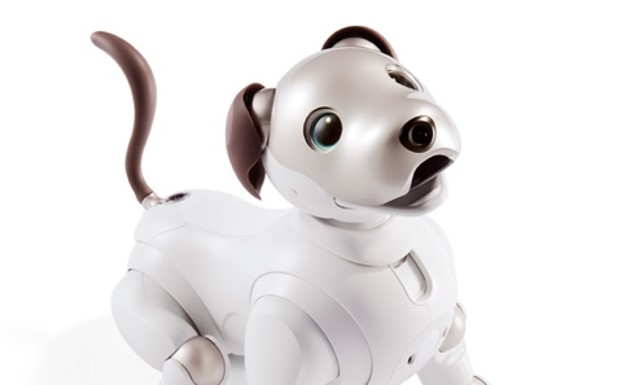
\includegraphics[keepaspectratio,width=4cm,clip]{images/previous_robots/aibo.jpg}
    \subcaption{aibo~\cite{web_aibo}}
    \label{fig:aibo}
  \end{minipage}
  \begin{minipage}[c]{0.32\linewidth}
    \centering
    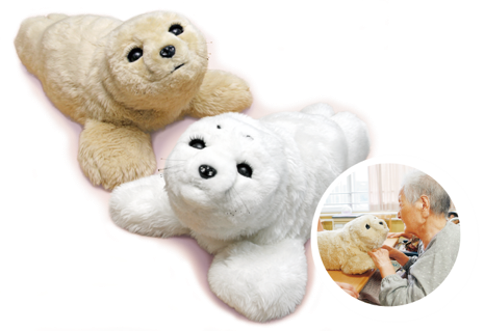
\includegraphics[keepaspectratio,width=4cm,clip]{images/previous_robots/paro.png}
    \subcaption{パロ~\cite{web_paro}}
    \label{fig:paro}
  \end{minipage}
  \begin{minipage}[c]{0.32\linewidth}
    \centering
    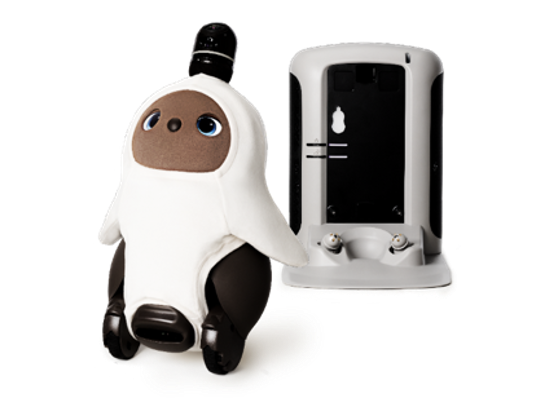
\includegraphics[keepaspectratio,width=4cm,clip]{images/previous_robots/lovot.png}
    \subcaption{LOVOT~\cite{web_lovot}}
    \label{fig:lovot}
  \end{minipage}
  \caption{愛玩用ロボットの例(高価格帯)}
  \label{fig:previous_robots_expensive}
\end{figure}

\begin{figure}[htbp]
  \centering
  \begin{minipage}[c]{0.32\linewidth}
    \centering
    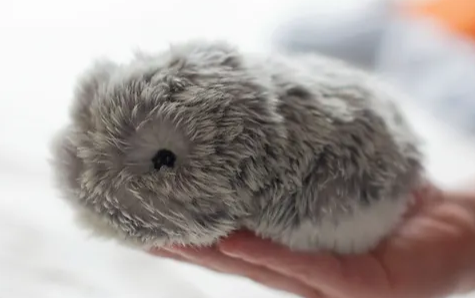
\includegraphics[keepaspectratio,width=4cm,clip]{images/previous_robots/moflin.png}
    \subcaption{Moflin~\cite{web_moflin}}
    \label{fig:moflin}
  \end{minipage}
  \begin{minipage}[c]{0.32\linewidth}
    \centering
    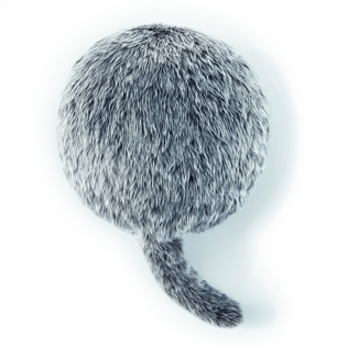
\includegraphics[keepaspectratio,width=4cm,clip]{images/previous_robots/qoobo.png}
    \subcaption{Qoobo~\cite{web_qoobo}}
    \label{fig:qoobo}
  \end{minipage}
  \begin{minipage}[c]{0.32\linewidth}
    \centering
    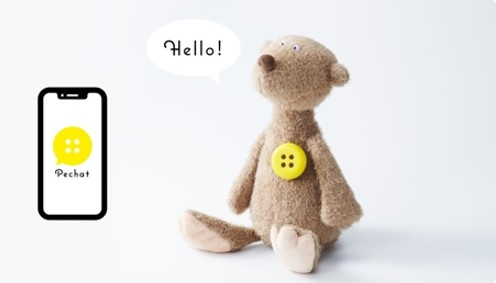
\includegraphics[keepaspectratio,width=4cm,clip]{images/previous_robots/pechat.jpg}
    \subcaption{pechat~\cite{web_pechat}}
    \label{fig:pechat}
  \end{minipage}
  \caption{愛玩用ロボットの例(低価格帯)}
  \label{fig:previous_robots_inexpensive}
\end{figure}


\subsection{ぬいぐるみの特徴}

そこで、人々に親しまれているぬいぐるみをロボットにすることを考える。
ぬいぐるみにはいくつかの特徴があるが、筆者の経験をもとにぬいぐるみの魅力を以下に述べる。

第一に、ぬいぐるみはその可愛らしい見た目ともふもふとした柔らかい触り心地から、落ち着きを与えてくれる。
幼い子どもがぬいぐるみとともに就寝するというのはよく見られる光景であろう。

次に、ぬいぐるみは自発的に動く存在ではなく、持ち主が触れ合いたいと考えたときだけ触れ合える。
これは、ぬいぐるみは持ち主の生活を縛らない、適度な距離感を持った愛玩対象であることを示す。
また、手入れの手間もほとんどかからないため、複数所持することは容易であり、使わない場合は長期間しまっておくことも可能である。

さらに、ぬいぐるみは人の心を投影する対象ともなりうる。
例えば(\figref{fig:mother})では女性が赤ちゃんにぬいぐるみを通して語りかけているが、これは女性の感情をぬいぐるみに代弁させているとも捉えられる。
つまり、ぬいぐるみとは愛玩対象であるとともに自身の代弁者ともなり、人とのコミュニケーションにおいて面と向かって伝えづらいこともぬいぐるみを通して語れるといった、コミュニケーションに彩りを持たせ、円滑に進める働きもある。

\begin{figure}[htbp]
  \centering
  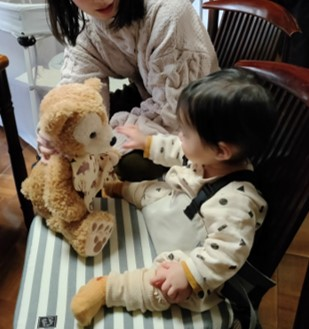
\includegraphics[width=6cm]{images/backgrounds/mother.jpg}
  \caption{ぬいぐるみを通して我が子に語り掛ける母親の様子}
  \label{fig:mother}
\end{figure}

最後に、ぬいぐるみは実に多様な見た目のものが存在する。
例えば本物の動物であれば、その大きさなどの物理的制約から、実際に飼育できるものは犬や猫、小動物といったものに限られる。
一方で、ぬいぐるみは多くの種類が存在し、より個人の好みに寄り添う存在となっている。
例えば(\figref{fig:zoo})ではアザラシやペンギン、ホッキョクグマなどを模したぬいぐるみが確認できるが、一つの店だけで50種類近くの品揃えがあることも珍しくない。
付け加えて重要なのが、これらのぬいぐるみはしばしば種々のイベントに合わせて贈られる文化が存在する点である。
子どもが誕生日に親からぬいぐるみを贈られたり、旅先の動物園や水族館、旅館等で土産に買ってもらったりすることは一般的な光景である。
そして、これらのぬいぐるみの多様性やそれにまつわる想い出は、目の前のぬいぐるみがオンリーワンの存在である印象を持ち主に与え、単なる布と綿からできた工業製品以上の愛着をもたらしうる。

\begin{figure}[htbp]
  \centering
  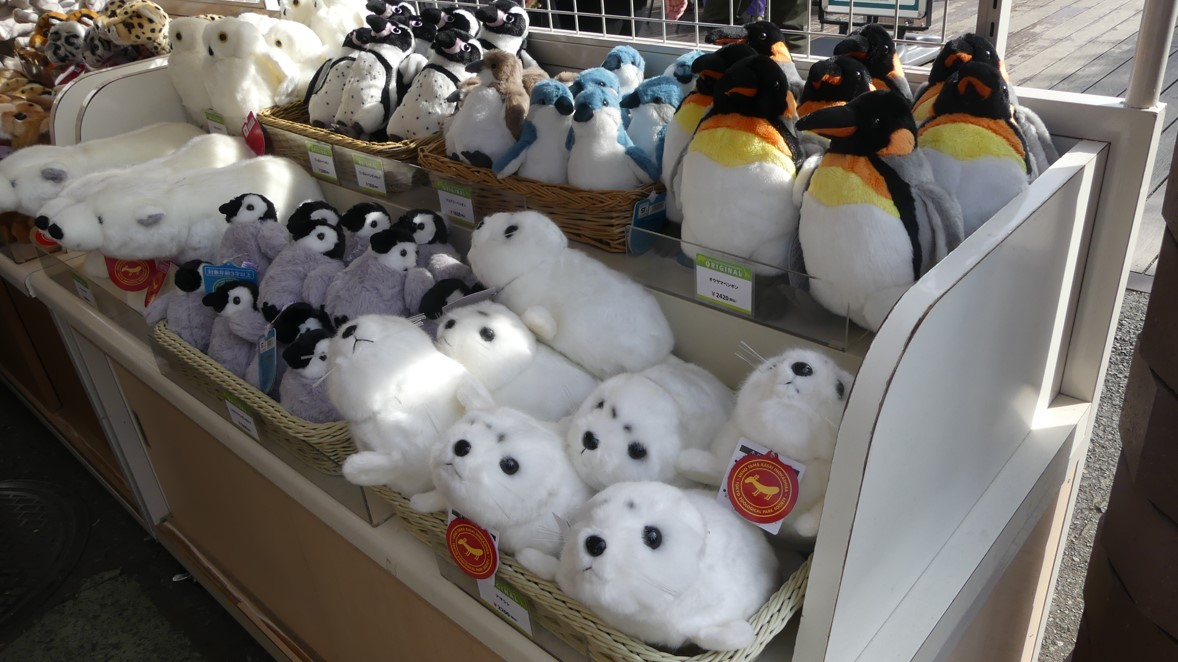
\includegraphics[width=8cm]{images/backgrounds/zoo.jpg}
  \caption{動物園でのぬいぐるみの販売風景}
  \label{fig:zoo}
\end{figure}

このように、ぬいぐるみには様々な魅力がある一方で、それらが逆に問題となることもある。
前述のとおり、ぬいぐるみは触れ合えいたいときだけ触れ合える存在であるが、裏を返せば持ち主の働きかけがない限り決して動かないことを意味し、愛玩対象としてはやや魅力に欠ける一面がある。

本プロジェクトでは、ぬいぐるみについて、その魅力を活かしつつも、さらなる愛着を抱ける対象に発展させることを目指した。
しかし、数多くの種類が存在するぬいぐるみについて、その一つ一つを独立した過程でロボット化することは開発コストの観点から現実的でない。
そこで、本プロジェクトでは複数の種類のぬいぐるみを効率的にロボット化できるモジュールを開発し、持ち主の好みに寄り添ったぬいぐるみが命を吹き込まれたかのように振る舞うシステムの構築を検討した。



\section{プロジェクト概要}
% ↓提案書コピペ
% 本プロジェクトではぬいぐるみ専用の組み込みAIモジュールを開発し、あらゆる種類のぬいぐるみにロボティクスを適用する。そして、幅広いぬいぐるみに効率的に知能を埋め込むためのプラットフォームの構築を目指す。

% ペットを飼うことは、現代においては非常に大きな決断となりうる。昔も今もペットに世話が必要なことは変わりない。しかし、特に犬や猫では現代特有の事情が絡んでくる。一つは、都市化が進み、ペットを飼いづらい環境になってきていることである。もう一つは、ペットの長寿命化である。医療の発展に伴い、犬や猫の寿命はこの数十年で飛躍的に伸びている。これは喜ばしい一方で、ペットを迎える行為が自身の今後15年の生活を左右する決断になったことを意味する。そういった背景も踏まえてか、近年では家庭用犬型ロボットなども販売され始めている。しかし、これらはペットとしての犬を意識しているためか、高機能な一方で価格が非常に高い。

% そこで本プロジェクトでは、機能を抑えた上でも違和感を最小限に止めるべく、普段は動くことのないぬいぐるみに知能を埋め込む方針でペットロボットを開発しようと考えた。しかし、それでもぬいぐるみ固有の問題が生じる。
% ぬいぐるみとは究極的には自身の鏡である。つまりそれは自己を投影しうる対象であり、外見には人それぞれ好みがある。そして、事実として世の中には犬や猫、熊、うさぎ、ねずみなど、あらゆる種類のぬいぐるみが存在する。もしこれらすべてにロボティクスを適用しようとしても開発費が莫大となり現実的ではないし、いくつかについて実装しただけでは需要を満たしきれない。

% そこで本プロジェクトでは、ぬいぐるみのロボット化に特化した組み込みAIモジュールを開発し、ぬいぐるみの骨格の規格化を目指す。そして、ぬいぐるみの毛皮と骨格の開発過程を分離することで、幅広いぬいぐるみに効率的に知能を埋め込むための土台を築き上げる。

本プロジェクトではぬいぐるみ専用の組み込みAIモジュールを開発し、あらゆる種類のぬいぐるみにロボティクスを適用する。
そして、幅広いぬいぐるみに効率的に知能を埋め込むためのプラットフォームの構築を目指す。

情報化が進んだ現代においても、一人暮らしなどで人が孤独を感じることは多い。
心の癒やしとしてペットの飼育が考えられるが、一人暮らしで世話を行うことは難しい。
そういった背景も踏まえてか、近年では愛玩用ロボットなども販売され始めている。
しかし、これらは工業製品であるがゆえに同じ製品ならば見た目はどれも同じであり、オンリーワンの要素に乏しい。

そこで本プロジェクトでは、人が適度な距離感で触れ合え、かつ多様な種類が存在するぬいぐるみに注目する。
そして、ぬいぐるみをロボット化することで現代の生活に即した心の癒やしを生み出そうと考えた。
しかし、ユーザの好みに応えるべく多くの種類が存在するぬいぐるみをすべてロボット化することは開発コストの観点から難しい。

そこで本プロジェクトでは、ぬいぐるみのロボット化に特化した組み込みAIモジュールを開発し、ぬいぐるみの骨格の規格化を目指す。
そして、ぬいぐるみの毛皮と骨格の開発過程を分離することで、幅広いぬいぐるみに効率的に知能を埋め込むための土台を築き上げる。

\section{開発内容}
\subsection{ぬいぐるみロボットシステムMohuticsの構成}
本プロジェクトでは、ぬいぐるみロボットを大きく以下の三要素に分割する(\figref{fig:mohutics:concept})。
\begin{description}
  \item[MohuCore(もふこあ)] ロボットの機械的・電気的要素を含む共通化された骨格部分
  \item[MohuKawa(もふかわ)] ロボットの内部骨格MohuCoreを覆うぬいぐるみ(毛皮)部分
  \item[MohuAI(もふあい)] ロボットに書き込むソフトウェア(知能)部分
\end{description}

\begin{figure}[htbp]
  \centering
  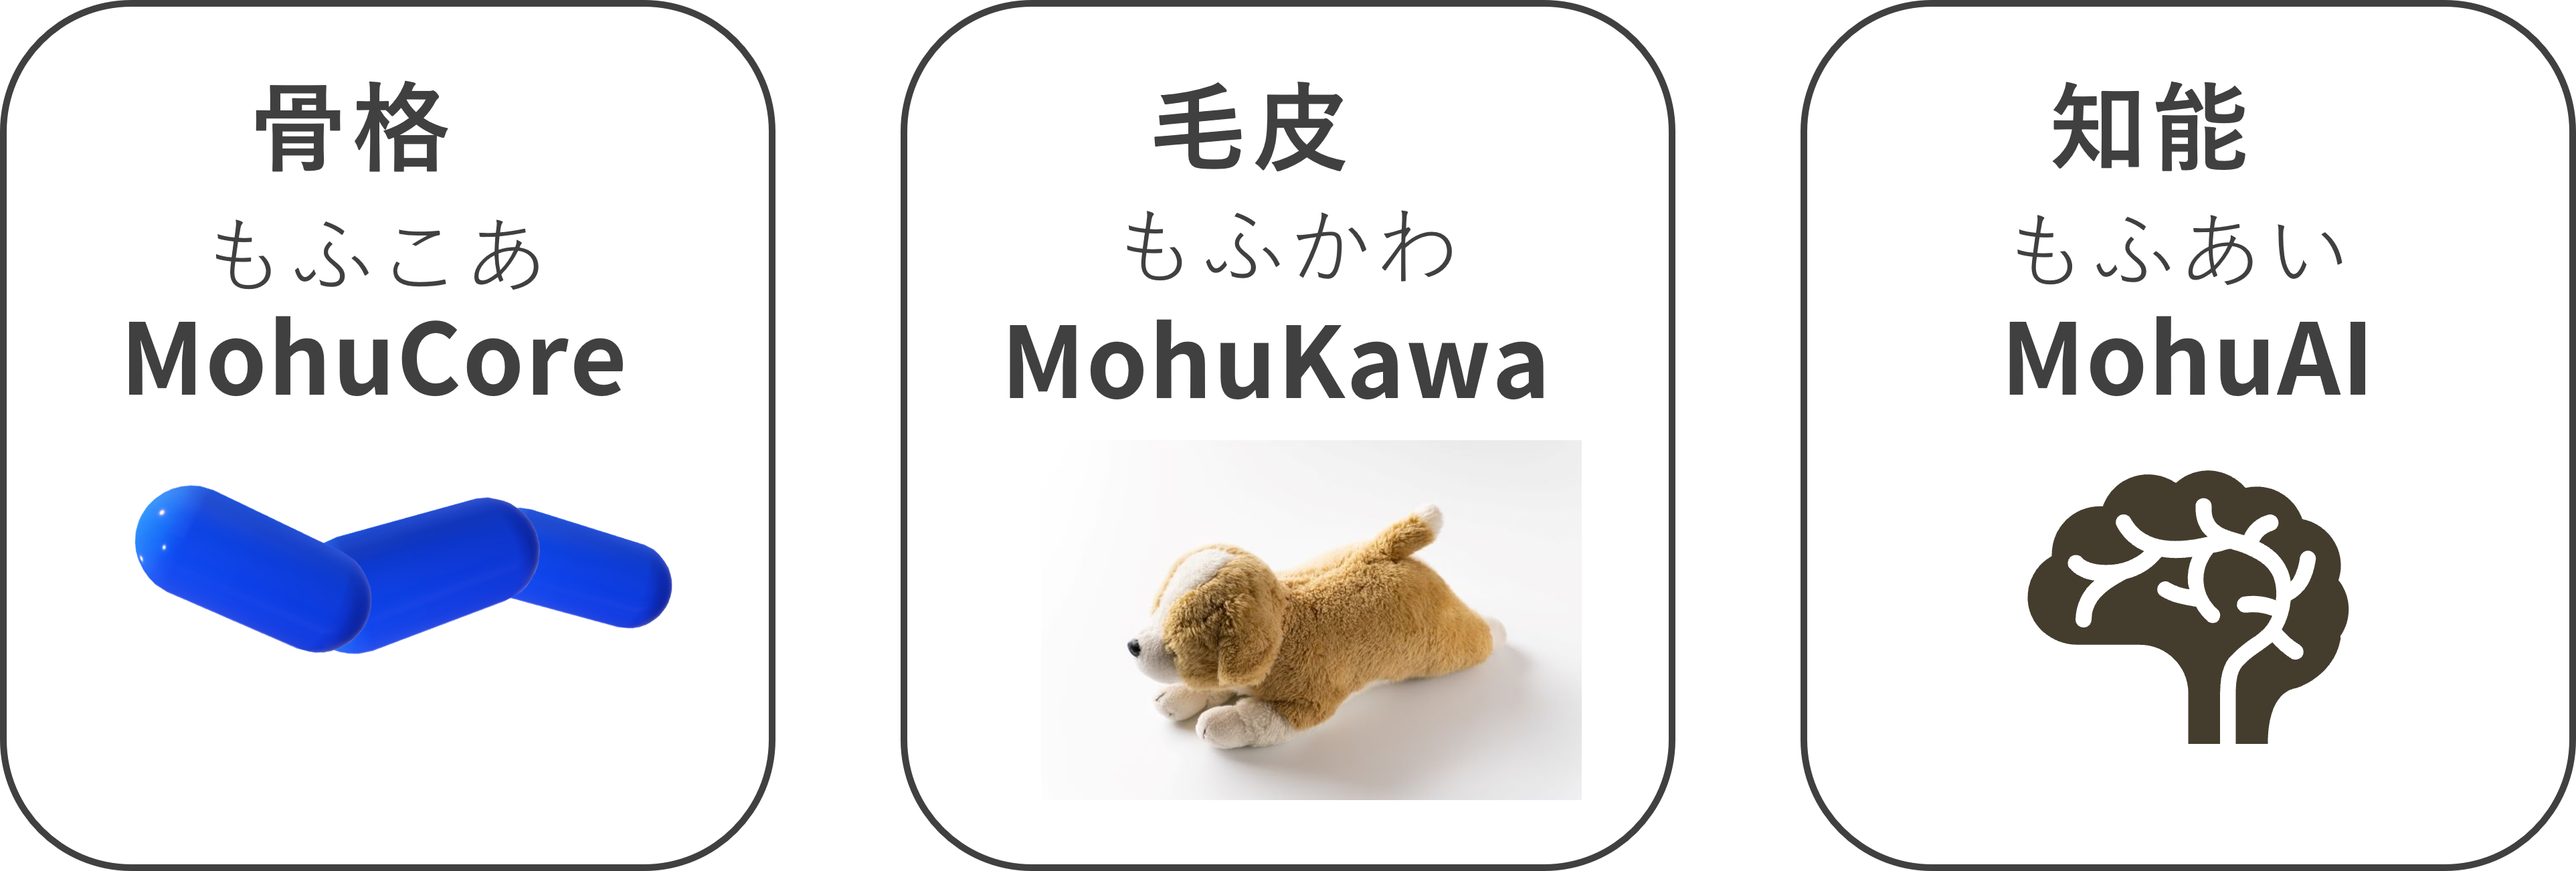
\includegraphics[width=12cm]{images/mohutics/concept.png}
  \caption{Mohuticsの構成}
  \label{fig:mohutics:concept}
\end{figure}

そして、開発の難所となるロボットのハードウェアやソフトウェアの共通化を進めることで、あらゆるぬいぐるみを効率的にロボット化することを目指した。

具体的には、まずはぬいぐるみロボットのセンサやアクチュエータ、制御基板等が含まれるロボットの骨格となるハードウェア部分MohuCoreを製作する。
ここで、MohuCoreは異なるぬいぐるみに接続可能な共通のハードウェアである点に注意する。

次に、ロボットの骨格MohuCoreを覆うようなぬいぐるみMohuKawaを製作する。
MohuKawaはぬいぐるみの外観に応じて犬やパンダなど、さまざまな種類が存在する。
しかし、これらにはすべて共通のジョイントが埋め込まれており、どの毛皮にも同じMohuCoreをその内部に組み込めるものとする。

さらに、ロボットに書き込むソフトウェアの総称をMohuAIとする。

そして、ユーザは共通の骨格MohuCoreと自分の好きなぬいぐるみの毛皮MohuKawaを用意し自ら組み合わせる(\figref{fig:mohutics:concept_embed})。
例えば、犬型のぬいぐるみに骨格を埋め込めば犬型のぬいぐるみロボットとなり(\figref{fig:mohutics:concept_dog})、熊型のぬいぐるみに同じ骨格を埋め込めば今度は熊型のぬいぐるみロボットとなる(\figref{fig:mohutics:concept_bear})。
最後に、ロボットのソフトウェアMohuAIを書き込むことで、自分の好きなぬいぐるみのロボットを簡単に手に入れることが可能となる。
\begin{figure}[htbp]
  \centering
  \begin{minipage}[c]{0.48\linewidth}
    \centering
    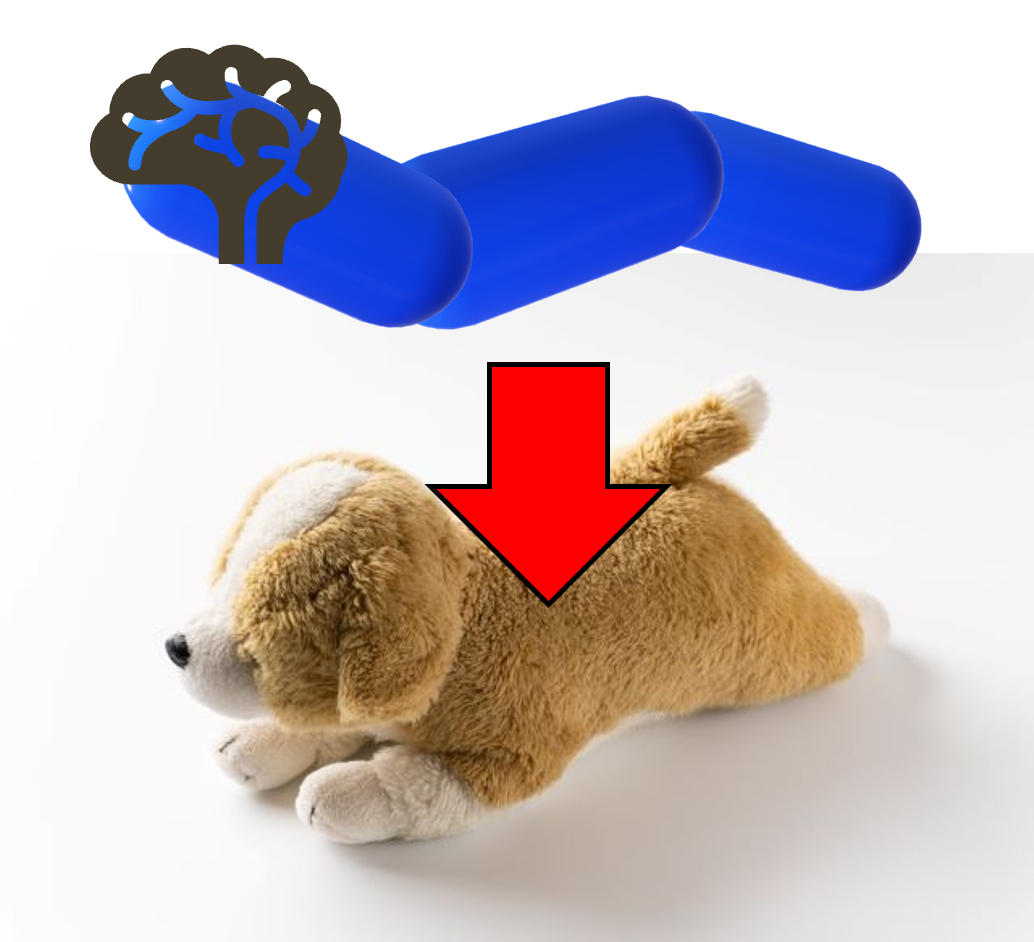
\includegraphics[keepaspectratio,width=4cm,clip]{images/mohutics/concept_dog.png}
    \subcaption{犬のぬいぐるみへの埋め込み}
    \label{fig:mohutics:concept_dog}
  \end{minipage}
  \begin{minipage}[c]{0.48\linewidth}
    \centering
    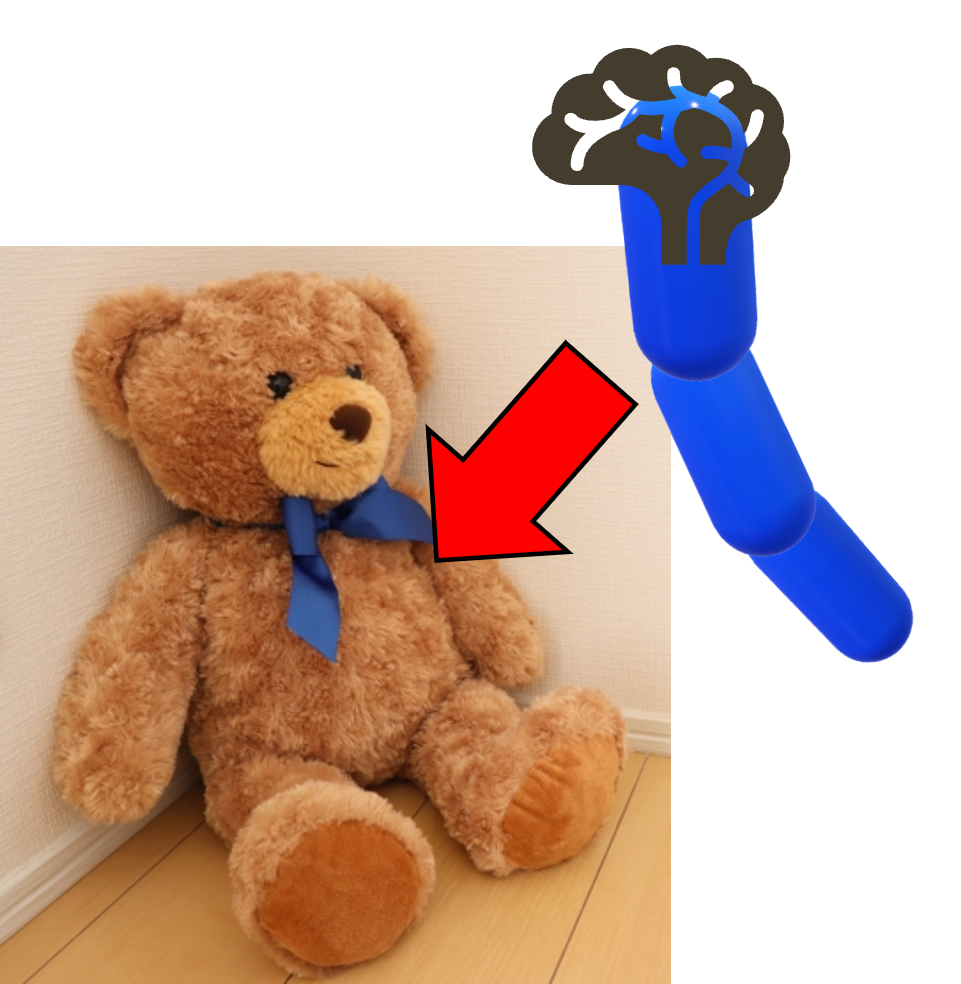
\includegraphics[keepaspectratio,width=4cm,clip]{images/mohutics/concept_bear.png}
    \subcaption{熊のぬいぐるみへの埋め込み}
    \label{fig:mohutics:concept_bear}
  \end{minipage}
  \caption{共通骨格を異なるぬいぐるみに埋め込む概念図}
  \label{fig:mohutics:concept_embed}
\end{figure}
以下では本プロジェクトで開発したMohuCore・MohuKawa・MohuAIそれぞれについて、その開発過程や機能をまとめる。

また、本プロジェクトで製作したぬいぐるみロボットMohuticsについて、複数のユーザに実際に触れ合ってもらい、聞き取りを行った。
その際のユーザからの評価についても記す。

\subsection{骨格MohuCoreの開発}
\subsubsection{関節の配置の検討}
本プロジェクトのぬいぐるみロボットではぬいぐるみロボットの骨格を共通化することが求められる。
まずは動作を行うために必要なアクチュエータの種類と配置について検討を行った。

家電量販店等では犬型の電動で歩くおもちゃが販売されている(\figref{fig:dog_toy:body})。
このおもちゃを分解したところ、おもちゃ内部に樹脂製の骨格があり、一つのモータとギヤ、クラッチ等を使ってからくり人形のように機械仕掛けで動いていることがわかった(\figref{fig:dog_toy:skeleton})。
\begin{figure}[htbp]
  \centering
  \begin{minipage}[c]{0.48\linewidth}
    \centering
    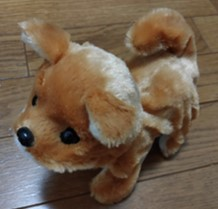
\includegraphics[keepaspectratio,width=4cm,clip]{images/dog_toy/dog.jpg}
    \subcaption{外観}
    \label{fig:dog_toy:body}
  \end{minipage}
  \begin{minipage}[c]{0.48\linewidth}
    \centering
    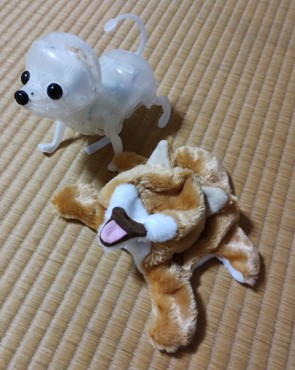
\includegraphics[keepaspectratio,width=4cm,clip]{images/dog_toy/skeleton.jpg}
    \subcaption{内部骨格と毛皮}
    \label{fig:dog_toy:skeleton}
  \end{minipage}
  \caption{市販の電動犬型おもちゃ}
  \label{fig:dog_toy}
\end{figure}

しかし、ギヤやクラッチを多用するとロボットとして関節を自由に動かすことは難しくなる。
よって、本プロジェクトのMohuCoreでは単純な回転軸を複数配置することとした。

モータの配置について、例えば(\figref{fig:mohucore:rot_animal})のような犬型やカンガルー型のぬいぐるみに共通の骨格を埋め込むことを考える。
これらの動物について、四肢に関節を埋め込んでぬいぐるみの脚を複雑に動かすことも可能であるが、骨格の構造を複雑にすればするほどぬいぐるみの形状に制約が生まれ、様々な種類のぬいぐるみに埋め込むことが難しくなってしまう。
よって、本プロジェクトではロボットを実際の動物の動きに近づけるのではなく、ぬいぐるみロボットとして必要十分な形状を目指し、最終的にMohuCoreは(\figref{fig:mohucore:serial_link})のような5関節のシリアルリンクロボットにした。
この構成では、例えば犬型ロボットの場合、頭が2自由度、腹の回転が1自由度、腰の回転が2自由度存在することになる。
本物の動物のように脚を自由に動かすことはできないが、ぬいぐるみロボットというコンセプトの下では十分に機能すると判断した。

\begin{figure}[htbp]
  \centering
  \begin{minipage}[c]{0.48\linewidth}
    \centering
    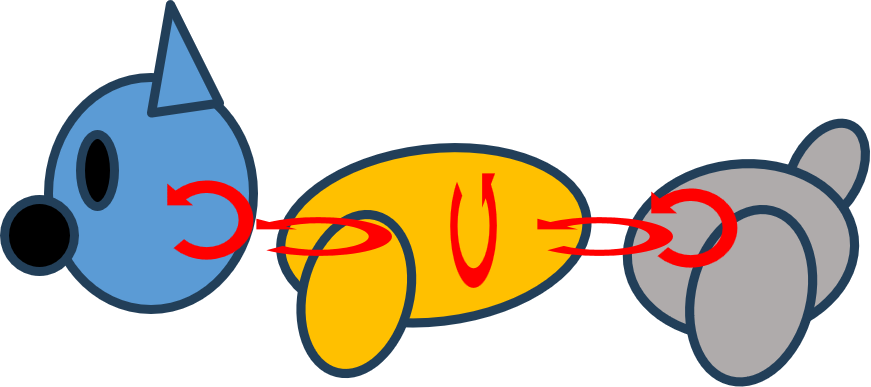
\includegraphics[keepaspectratio,width=4cm,clip]{images/mohucore/rot_dog.png}
    \subcaption{犬型}
    \label{fig:mohucore:rot_dog}
  \end{minipage}
  \begin{minipage}[c]{0.48\linewidth}
    \centering
    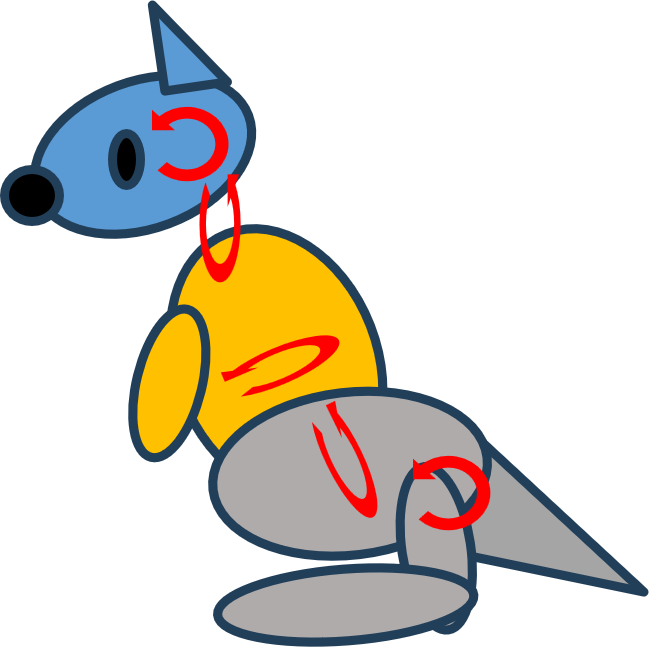
\includegraphics[keepaspectratio,width=4cm,clip]{images/mohucore/rot_kangaroo.png}
    \subcaption{カンガルー型}
    \label{fig:mohucore:rot_kangaroo}
  \end{minipage}
  \caption{サーボモータの回転軸の配置の検討}
  \label{fig:mohucore:rot_animal}
\end{figure}

\begin{figure}[htbp]
  \centering
  \begin{minipage}[c]{0.48\linewidth}
    \centering
    \includegraphics[keepaspectratio,width=6cm,clip]{images/mohucore/5motors.png}
    \subcaption{シリアルリンクの模式図}
  \end{minipage}
  \begin{minipage}[c]{0.48\linewidth}
    \centering
    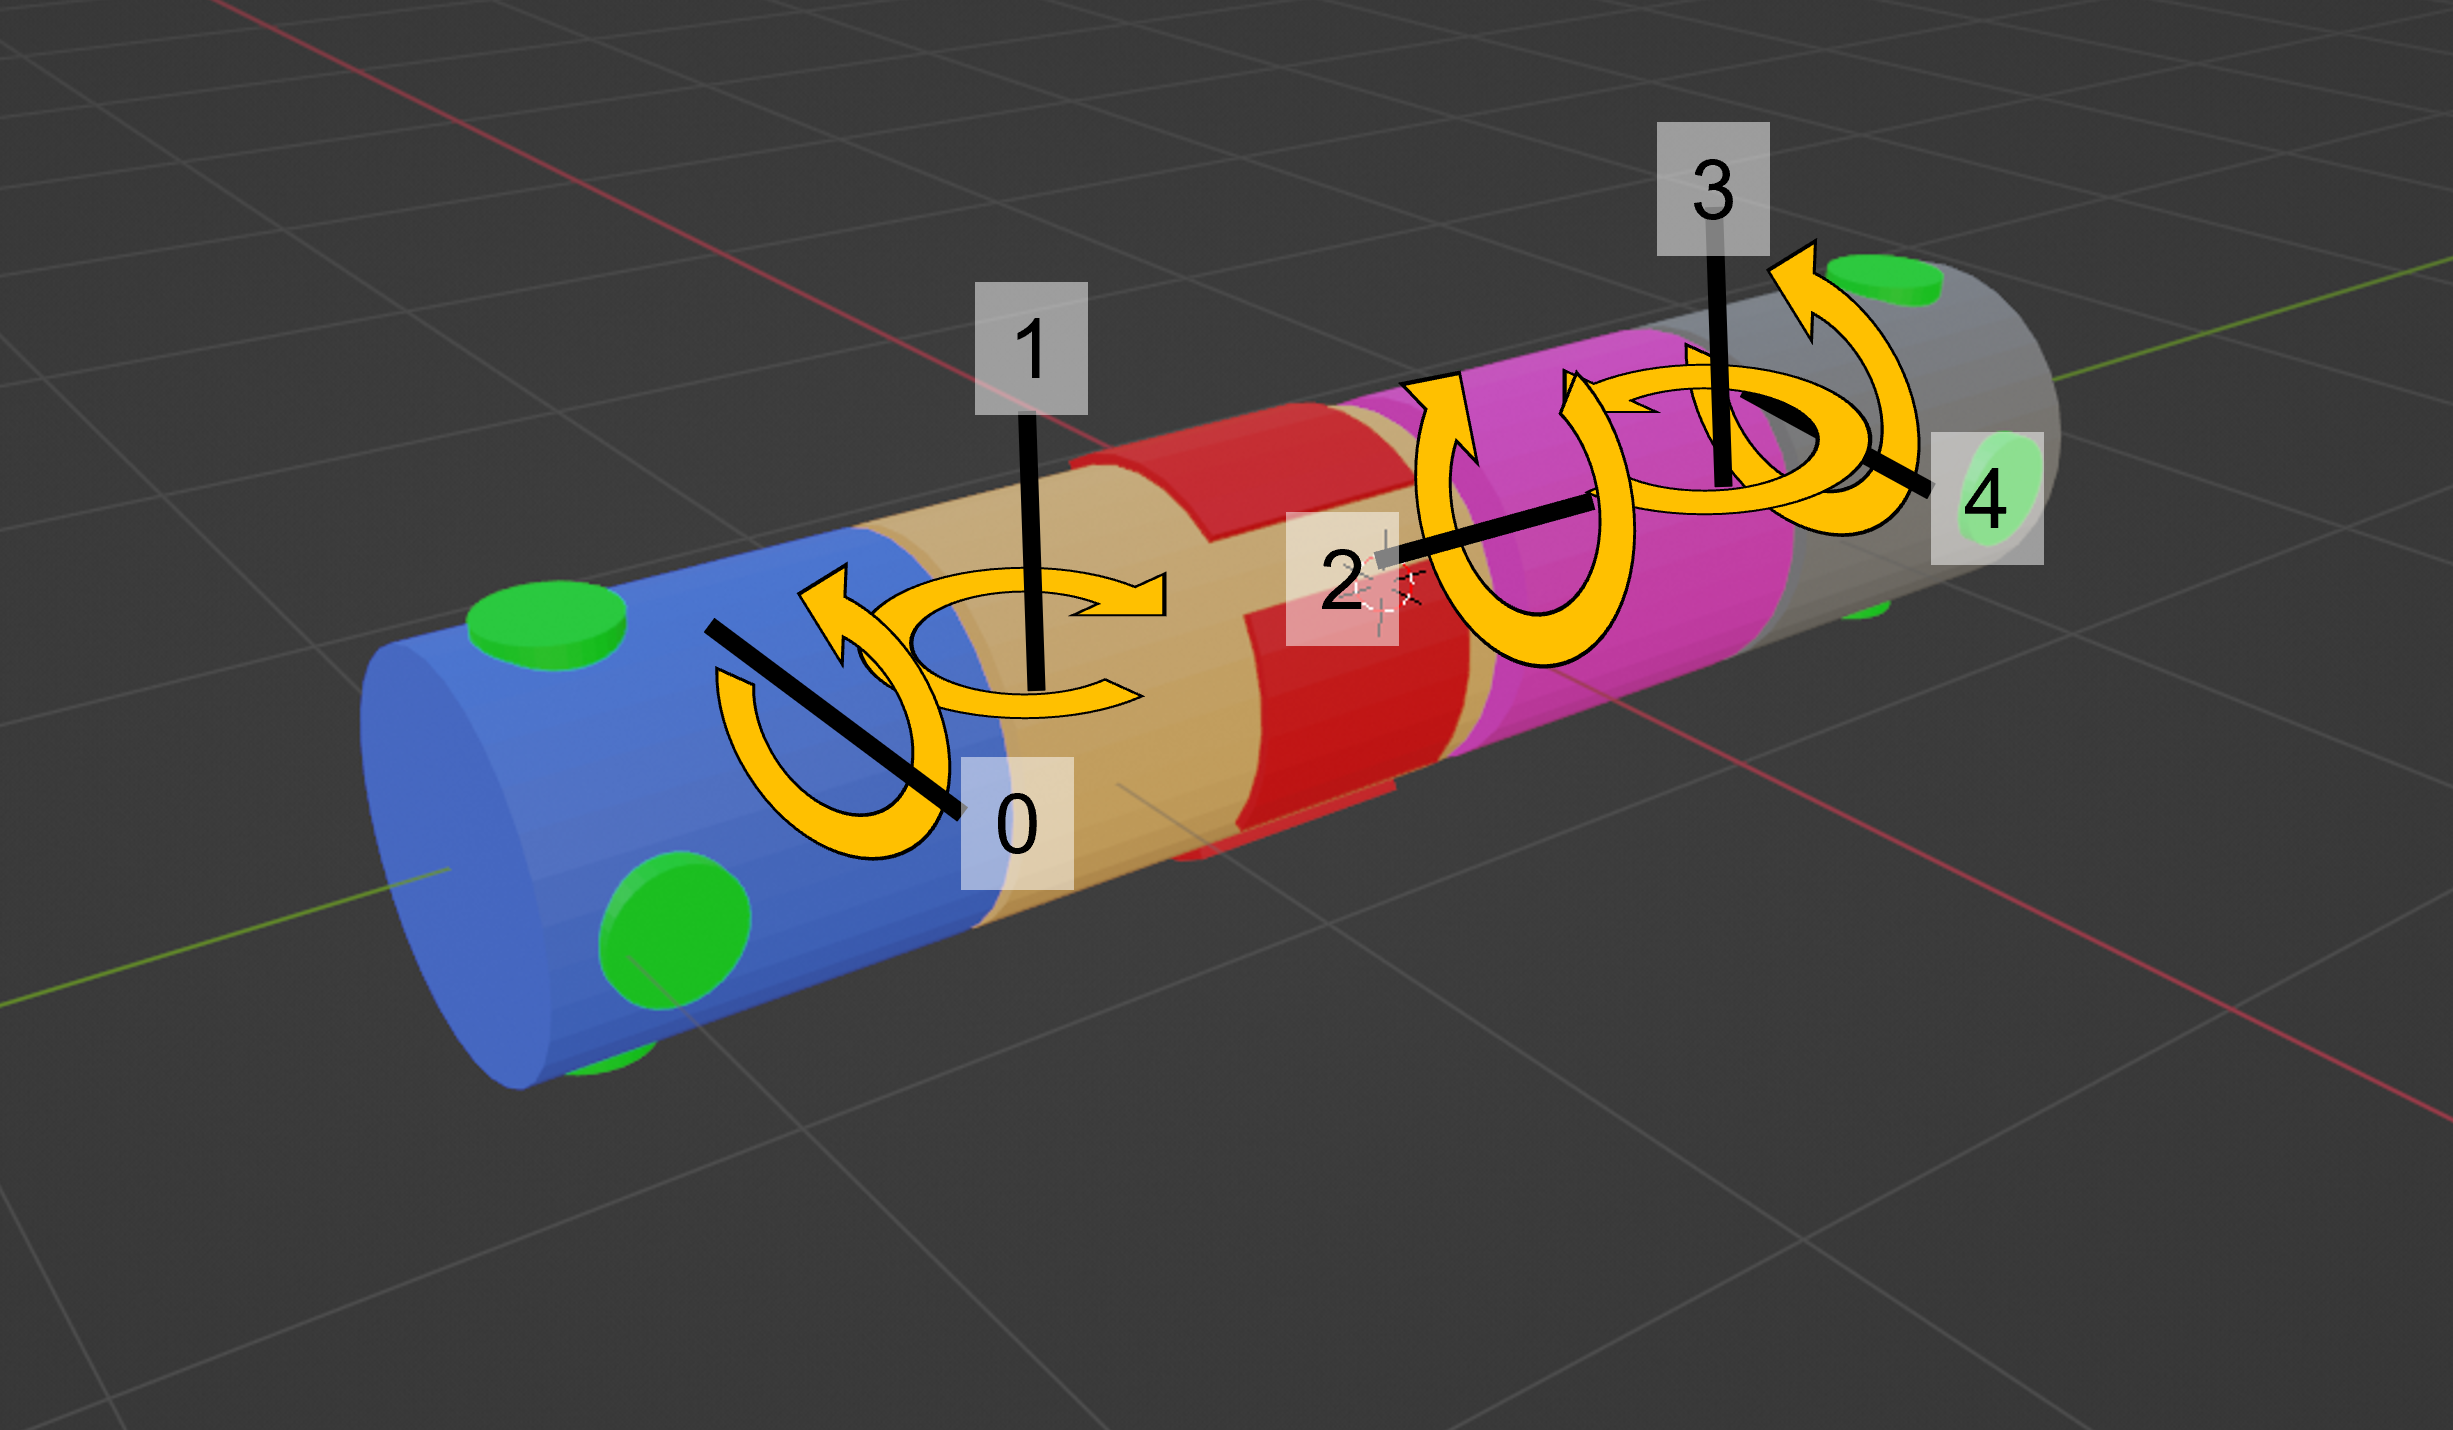
\includegraphics[keepaspectratio,width=6cm,clip]{images/mohucore/rot_arrangement.png}
    \subcaption{回転軸の配置}
  \end{minipage}
  \caption{MohuCoreのシリアルリンクの構造と回転軸の配置}
  \label{fig:mohucore:serial_link}
\end{figure}

\subsubsection{機械的要素の開発}
本プロジェクトのぬいぐるみロボットは実際の動物ではなくぬいぐるみの発展型としての愛玩用ロボットを目指している。
したがって、ロボットの関節をできだけ滑らかに動くように作り、少なくともロボットの電源が入っていないときは普通のぬいぐるみのようにユーザの抱く・曲げるといった動作に自然に追従することが望ましい。

アクチュエータについて、プロジェクト初期はギヤ比が1:30程度の比較的低ギヤ比のギヤボックスを使用することで、滑らかな回転を目指した(\figref{fig:prototype_01})。
しかし、この方法では各関節角を測定してフィードバック回路を構成する必要がある。
さらに、ぬいぐるみロボットではユーザがロボット本体を押さえつけることで各関節に大きなトルクが掛かる可能性がある。
その場合、モータやモータドライバの過熱を防ぐにはモータの電流制御も必要となり回路構成が非常に複雑になってしまう。

\begin{figure}[htbp]
  \centering
  \begin{minipage}[c]{0.64\linewidth}
    \centering
    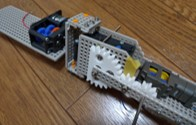
\includegraphics[keepaspectratio,width=8cm,clip]{images/prototype/prototype_01.png}
    \subcaption{関節の構造}
  \end{minipage}
  \begin{minipage}[c]{0.32\linewidth}
    \centering
    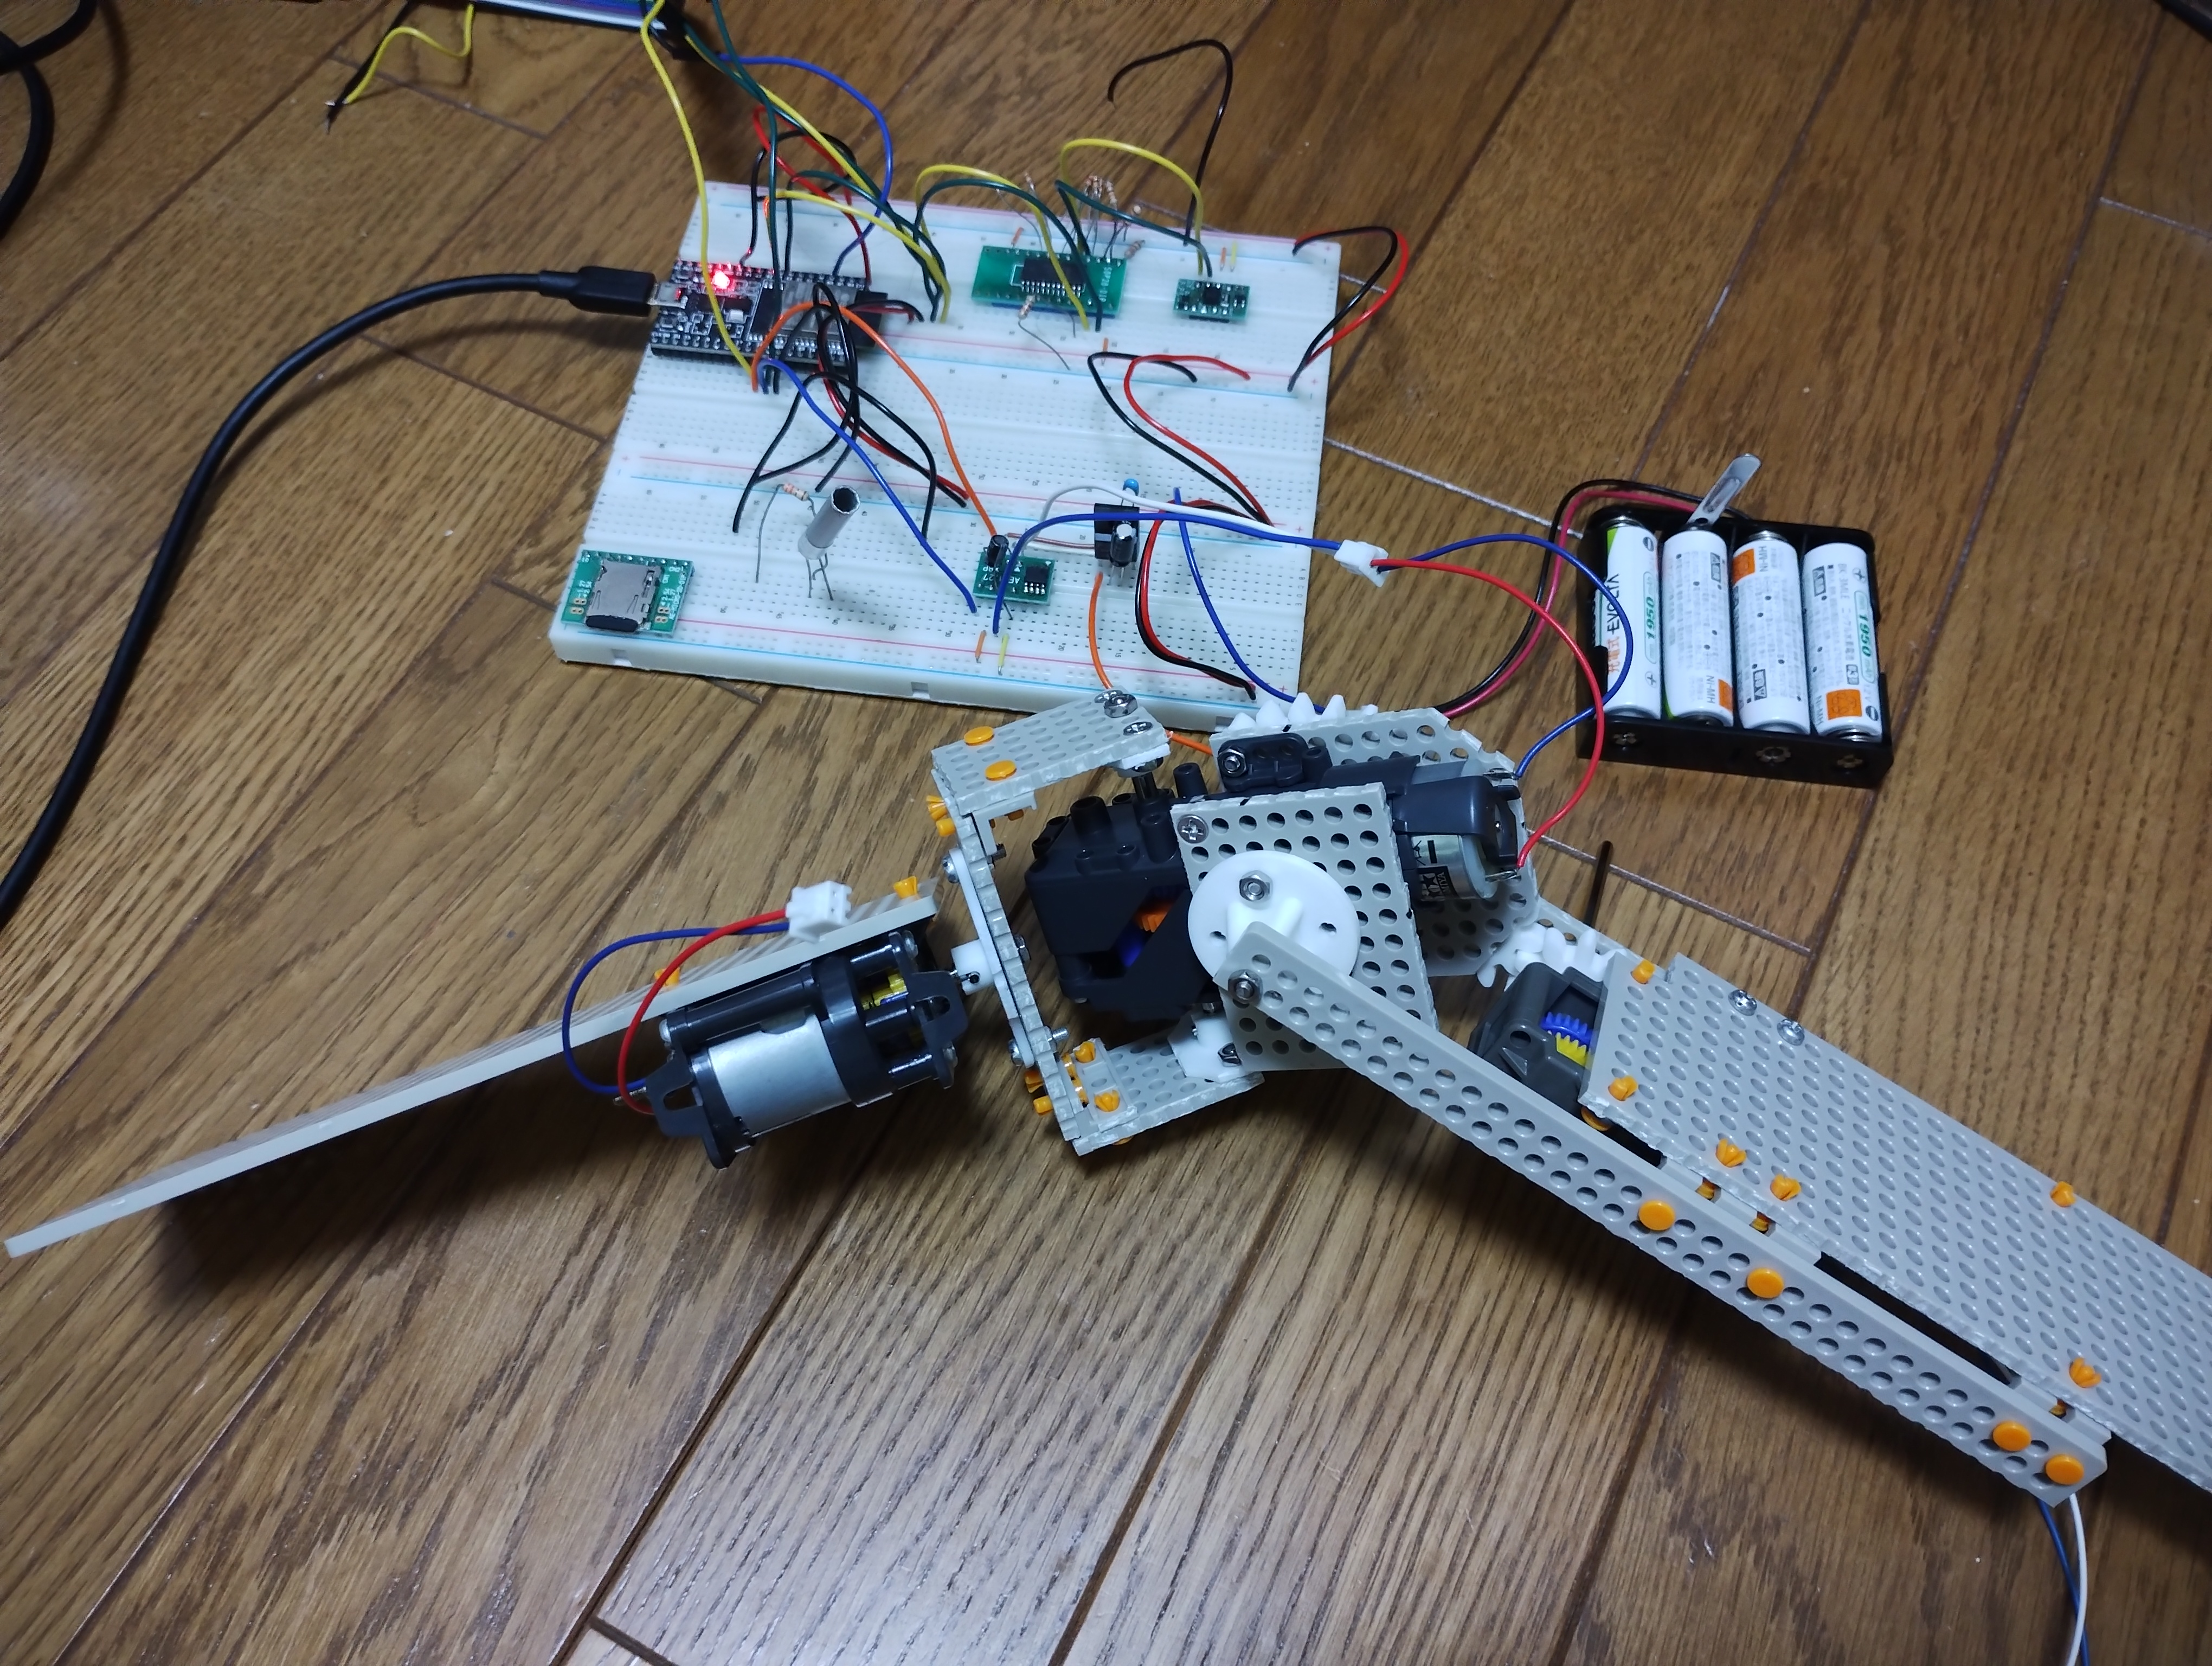
\includegraphics[keepaspectratio,width=4cm,clip]{images/prototype/prototype_01_circuit.jpg}
    \subcaption{回路試験の様子}
  \end{minipage}
  \caption{開発初期の低ギヤ比のギヤボックスを用いたMohuCoreの試作置}
  \label{fig:prototype_01}
\end{figure}

そこで、本プロジェクトのMohuCoreでは多少の動作の滑らかさは犠牲になるものの、実装を急ぐためにアクチュエータにラジコン等で使用されるサーボモータを使用することとした。
これにより、関節角をフィートバックする回路は不要となり、実装が素早く進むこととなった。
ただし、これでもモータの過熱等の問題は解決できておらず、\ref{sec:challenges}節で電流制御が行える高性能なサーボモータを使用した改良型について言及している(\figref{fig:prototype_04})。
サーボモータはMG996Rを使用し、関節配置が問題ないかを確認した(\figref{fig:prototype_02})。
そして、VU65塩ビパイプや3Dプリンタで製作した部品(\figref{fig:mohucore:cad})を組み立てて、MohuCoreの基本骨格とした(\figref{fig:mohucore:skeleton})。
MohuCoreは直径約8cm、長さ約40cmの円筒型である。

\begin{figure}[htbp]
  \centering
  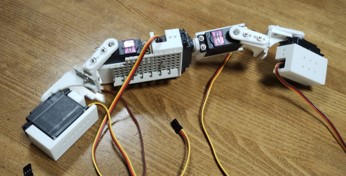
\includegraphics[width=8cm]{images/prototype/prototype_02.jpg}
  \caption{サーボモータの関節配置の検討に用いた試作}
  \label{fig:prototype_02}
\end{figure}

\begin{figure}[htbp]
  \centering
  \begin{minipage}[c]{0.32\linewidth}
    \centering
    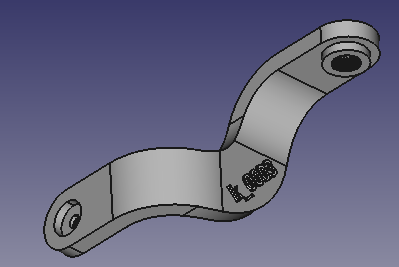
\includegraphics[keepaspectratio,width=4cm,clip]{images/mohucore/part_k.png}
  \end{minipage}
  \begin{minipage}[c]{0.32\linewidth}
    \centering
    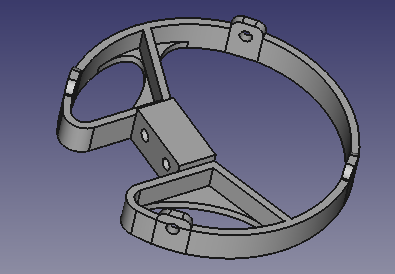
\includegraphics[keepaspectratio,width=4cm,clip]{images/mohucore/part_l.png}
  \end{minipage}
  \begin{minipage}[c]{0.32\linewidth}
    \centering
    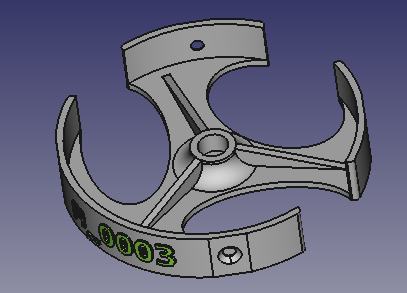
\includegraphics[keepaspectratio,width=4cm,clip]{images/mohucore/part_m.png}
  \end{minipage}
  \caption{3DCADによるMohuCoreの部品の設計}
  \label{fig:mohucore:cad}
\end{figure}

\begin{figure}[htbp]
  \centering
  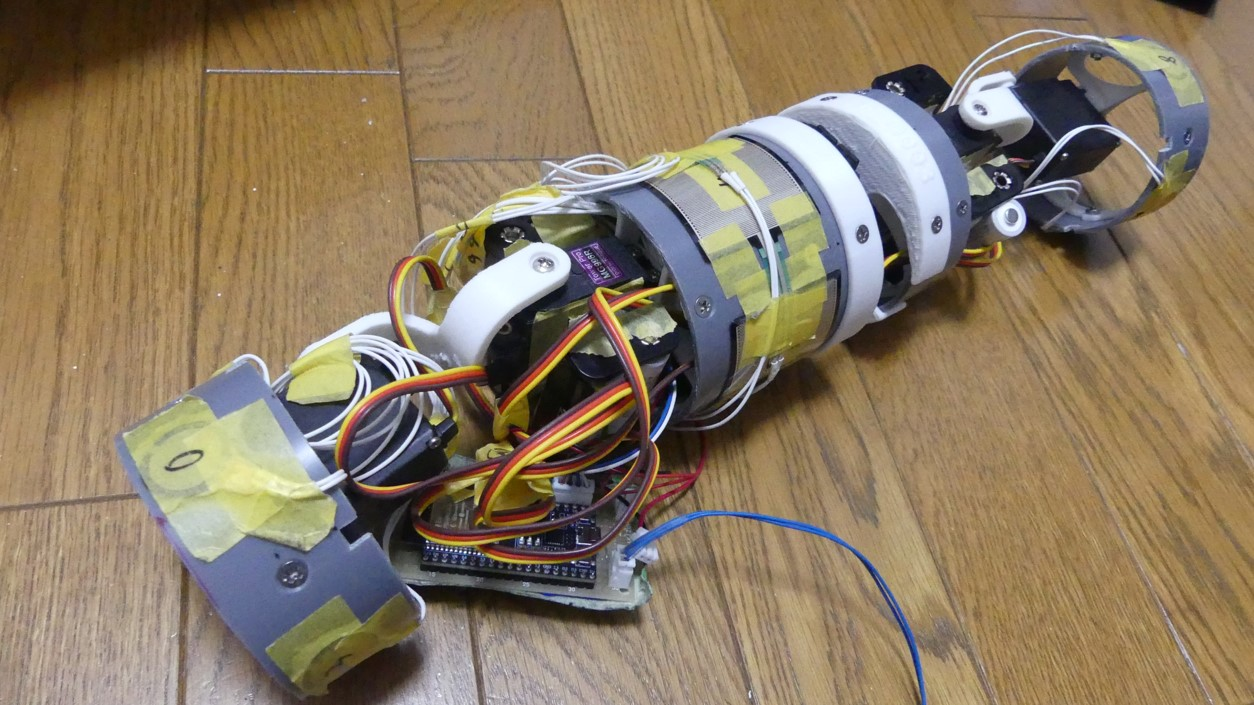
\includegraphics[width=8cm]{images/mohucore/skeleton.jpg}
  \caption{MohuCoreの外観}
  \label{fig:mohucore:skeleton}
\end{figure}

\subsubsection{電気的要素の開発}
ロボットを制御するためのCPUとして、当初はぬいぐるみロボットとして長時間触れ合えるよう、消費電力の少なさに焦点を置いていた。
市販の高性能な愛玩用ロボットは一回の充電で2時間程度しか動き回れないという。
ぬいぐるみロボットであれば処理性能より消費電力を抑えて長時間楽しめる方が価値があると考えた。
そこで開発初期はNuttXというリアルタイムOSが使用可能なSpresense~\cite{web_spresense}というマイコンボードを使用して開発を進めた。
しかし、NuttXがマイコンボードのすべての機能には対応していない点とSpresenseの特徴的な機能(GPS・ハイレゾリューションオーディオ処理など)がぬいぐるみロボットに求められる性能からはやや離れていたため、CPUの変更を決断した。

本プロジェクトでは、最終的にESP32-DevkitCというマイコンボードを使用した。
このマイコンは処理性能は高くないものの、IoT開発に適したWi-Fi等の無線機能や豊富な入出力端子などを備えている。
開発環境には公式開発環境のESP-IDFを採用した。
なお、CPU等もモータと同じく\ref{sec:challenges}節で改良型に言及している。

ロボットに埋め込むセンサとしては、9軸姿勢センサBNO055と感圧センサを採用した。
BNO055は加速度・地磁気・角速度・相対的な姿勢Quaternion情報が得られる姿勢センサであり、ぬいぐるみロボットの振動や姿勢情報を取得できる。
感圧センサはセンサ表面の圧力に応じて抵抗値が変わるセンサであり、ぬいぐるみを抱きしめた強さを測定できる。
感圧センサはロボットの骨格MohuCore表面に12個配置したが、多数のAD変換器が必要なため、PIC16F18444というマイコンを使用して簡易的なAD変換器を実装した(\figref{fig:mohucore:sensor})。
そして、これらの姿勢センサやPICマイコンからの信号は\(\mathrm{I^2C}\)通信でESP32と接続されている。
電源には単3型ニッケル水素二次充電池を使用した。

\begin{figure}[htbp]
  \centering
  \begin{minipage}[c]{0.64\linewidth}
    \centering
    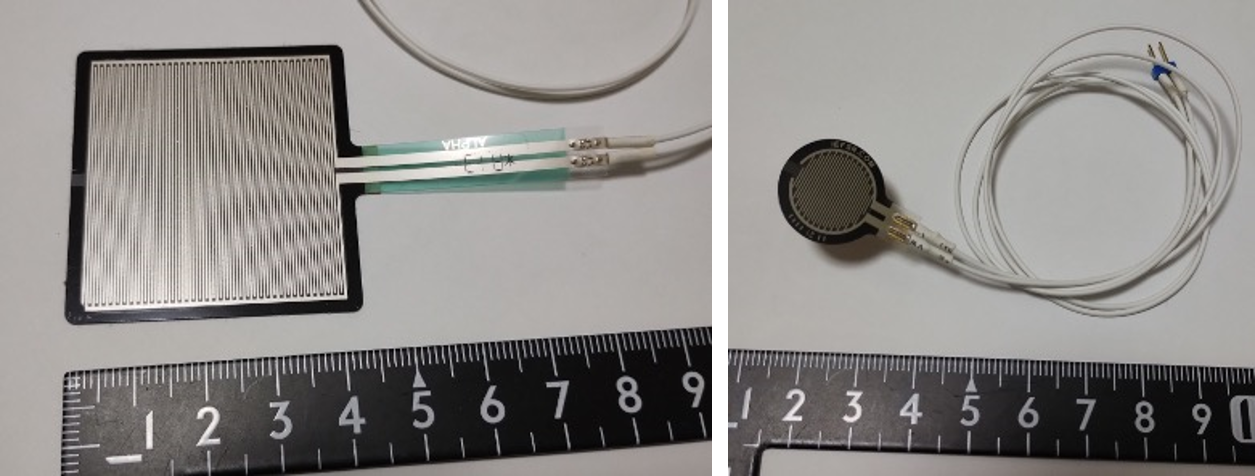
\includegraphics[keepaspectratio,width=8cm,clip]{images/mohucore/touch_sensor.png}
    \subcaption{感圧センサ}
  \end{minipage}
  \begin{minipage}[c]{0.32\linewidth}
    \centering
    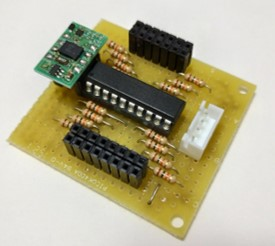
\includegraphics[keepaspectratio,width=4cm,clip]{images/mohucore/sensor_board.jpg}
    \subcaption{姿勢センサとPICマイコンを収めたセンサボード}
  \end{minipage}
  \caption{MohuCoreに取り付けられたセンサ}
  \label{fig:mohucore:sensor}
\end{figure}


\subsection{毛皮MohuKawaの開発}

ロボットのぬいぐるみ部分となるMohuKawaについては、大きく分けて以下の二つの方法で製作した。
\begin{description}
  \item[ぬいぐるみを展開図から完全新規設計]犬型
  \item[市販のぬいぐるみをMohutics対応形状に改造]人型・アナゴ型・パンダ型  
\end{description}

本プロジェクトのために完全新規設計したぬいぐるみとしては、犬型のぬいぐるみを用意した。
Mohuticsではぬいぐるみの内部に骨格となるMohuCoreを埋め込む必要があるため、ぬいぐるみ自体をMohuCoreに合わせて製作することが望ましい。
よって、犬型のぬいぐるみについては筆者が展開図の設計から縫製までをすべて行った。

一方で、世の中にはすでに数多くのぬいぐるみが存在するため、ユーザによってはすでに存在するぬいぐるみを使用したい場合があると想定される。
また、後述するとおり、ぬいぐるみの新規設計はやや難易度が高い。
そのため、ユーザの中には、手芸が得意で市販品の改造程度であれば問題なく行えるが新規設計するほどの時間や技術がないという者も一定数いると考えられる。
そこで、本プロジェクトでは新規設計のぬいぐるみだけでなく市販のぬいぐるみをMohuticsに対応するよう改造したものも製作した。
人型・アナゴ型・パンダ型のぬいぐるみは市販品の内部をくり貫くように加工している。

以下では、両者の方法について、その製作の過程や内容をまとめる。

\subsubsection{完全新規設計のMohuKawa}

犬型のぬいぐるみを設計するために、まずはオープンソースの3DCGソフトウェアであるBlenderを使用して犬のぬいぐるみのモデリングを行った(\figref{fig:mohukawa:blender_01})。
次に、BlenderのUV展開機能を使用して展開図を作成し(\figref{fig:mohukawa:uv})、厚紙に印刷するなどして型紙を製作した。
そして、生地を裁断してミシンで縫製し(\figref{fig:mohukawa:saw})、ポリエステル綿を詰めてぬいぐるみの形状に仕立てた。
最後に、3Dプリンタで製作したMohuCoreとMohuKawaを接続するためのジョイントを取り付け(\figref{fig:mohukawa:joint})、犬型のぬいぐるみとした(\figref{fig:mohukawa:dog})。
なお、このジョイントは十分な保持力は備えつつもあえてネジ等の締結器具は使わず、工具不要で簡単に取り外しができるよう設計されている。

\begin{figure}[htbp]
  \centering
  \begin{minipage}[c]{0.56\linewidth}
    \centering
    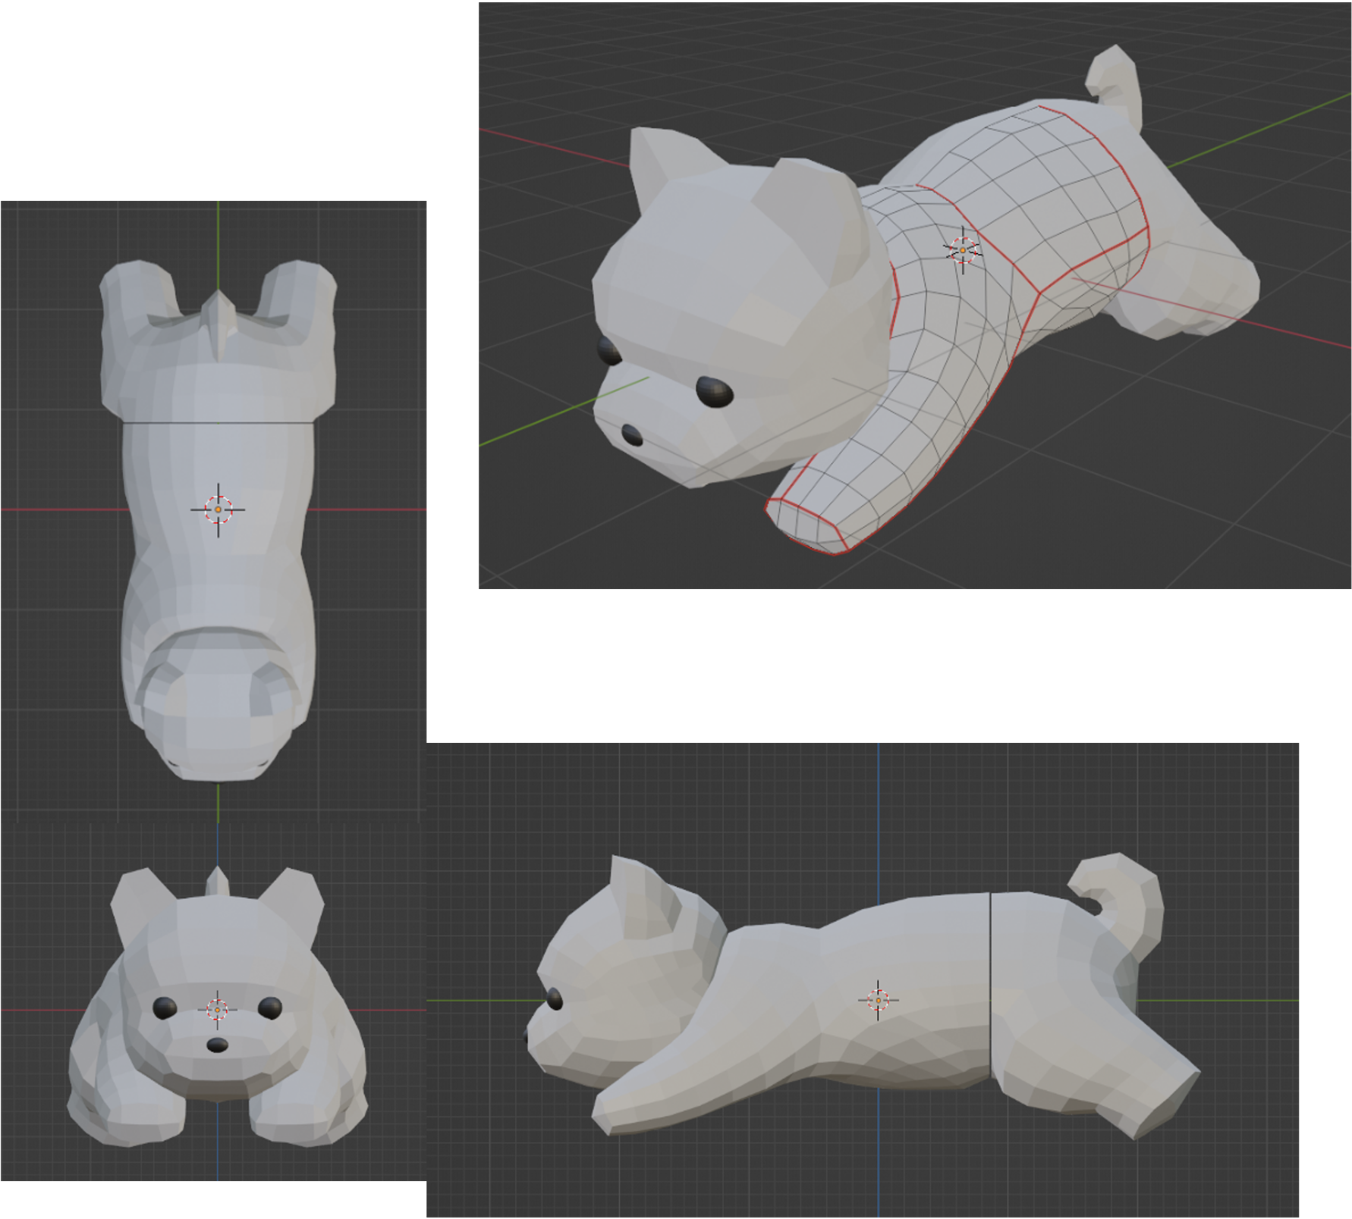
\includegraphics[keepaspectratio,width=8cm,clip]{images/mohukawa/blender_01.png}
    \subcaption{三面図}
    \label{fig:mohukawa:blender_01}
  \end{minipage}
  \begin{minipage}[c]{0.40\linewidth}
    \centering
    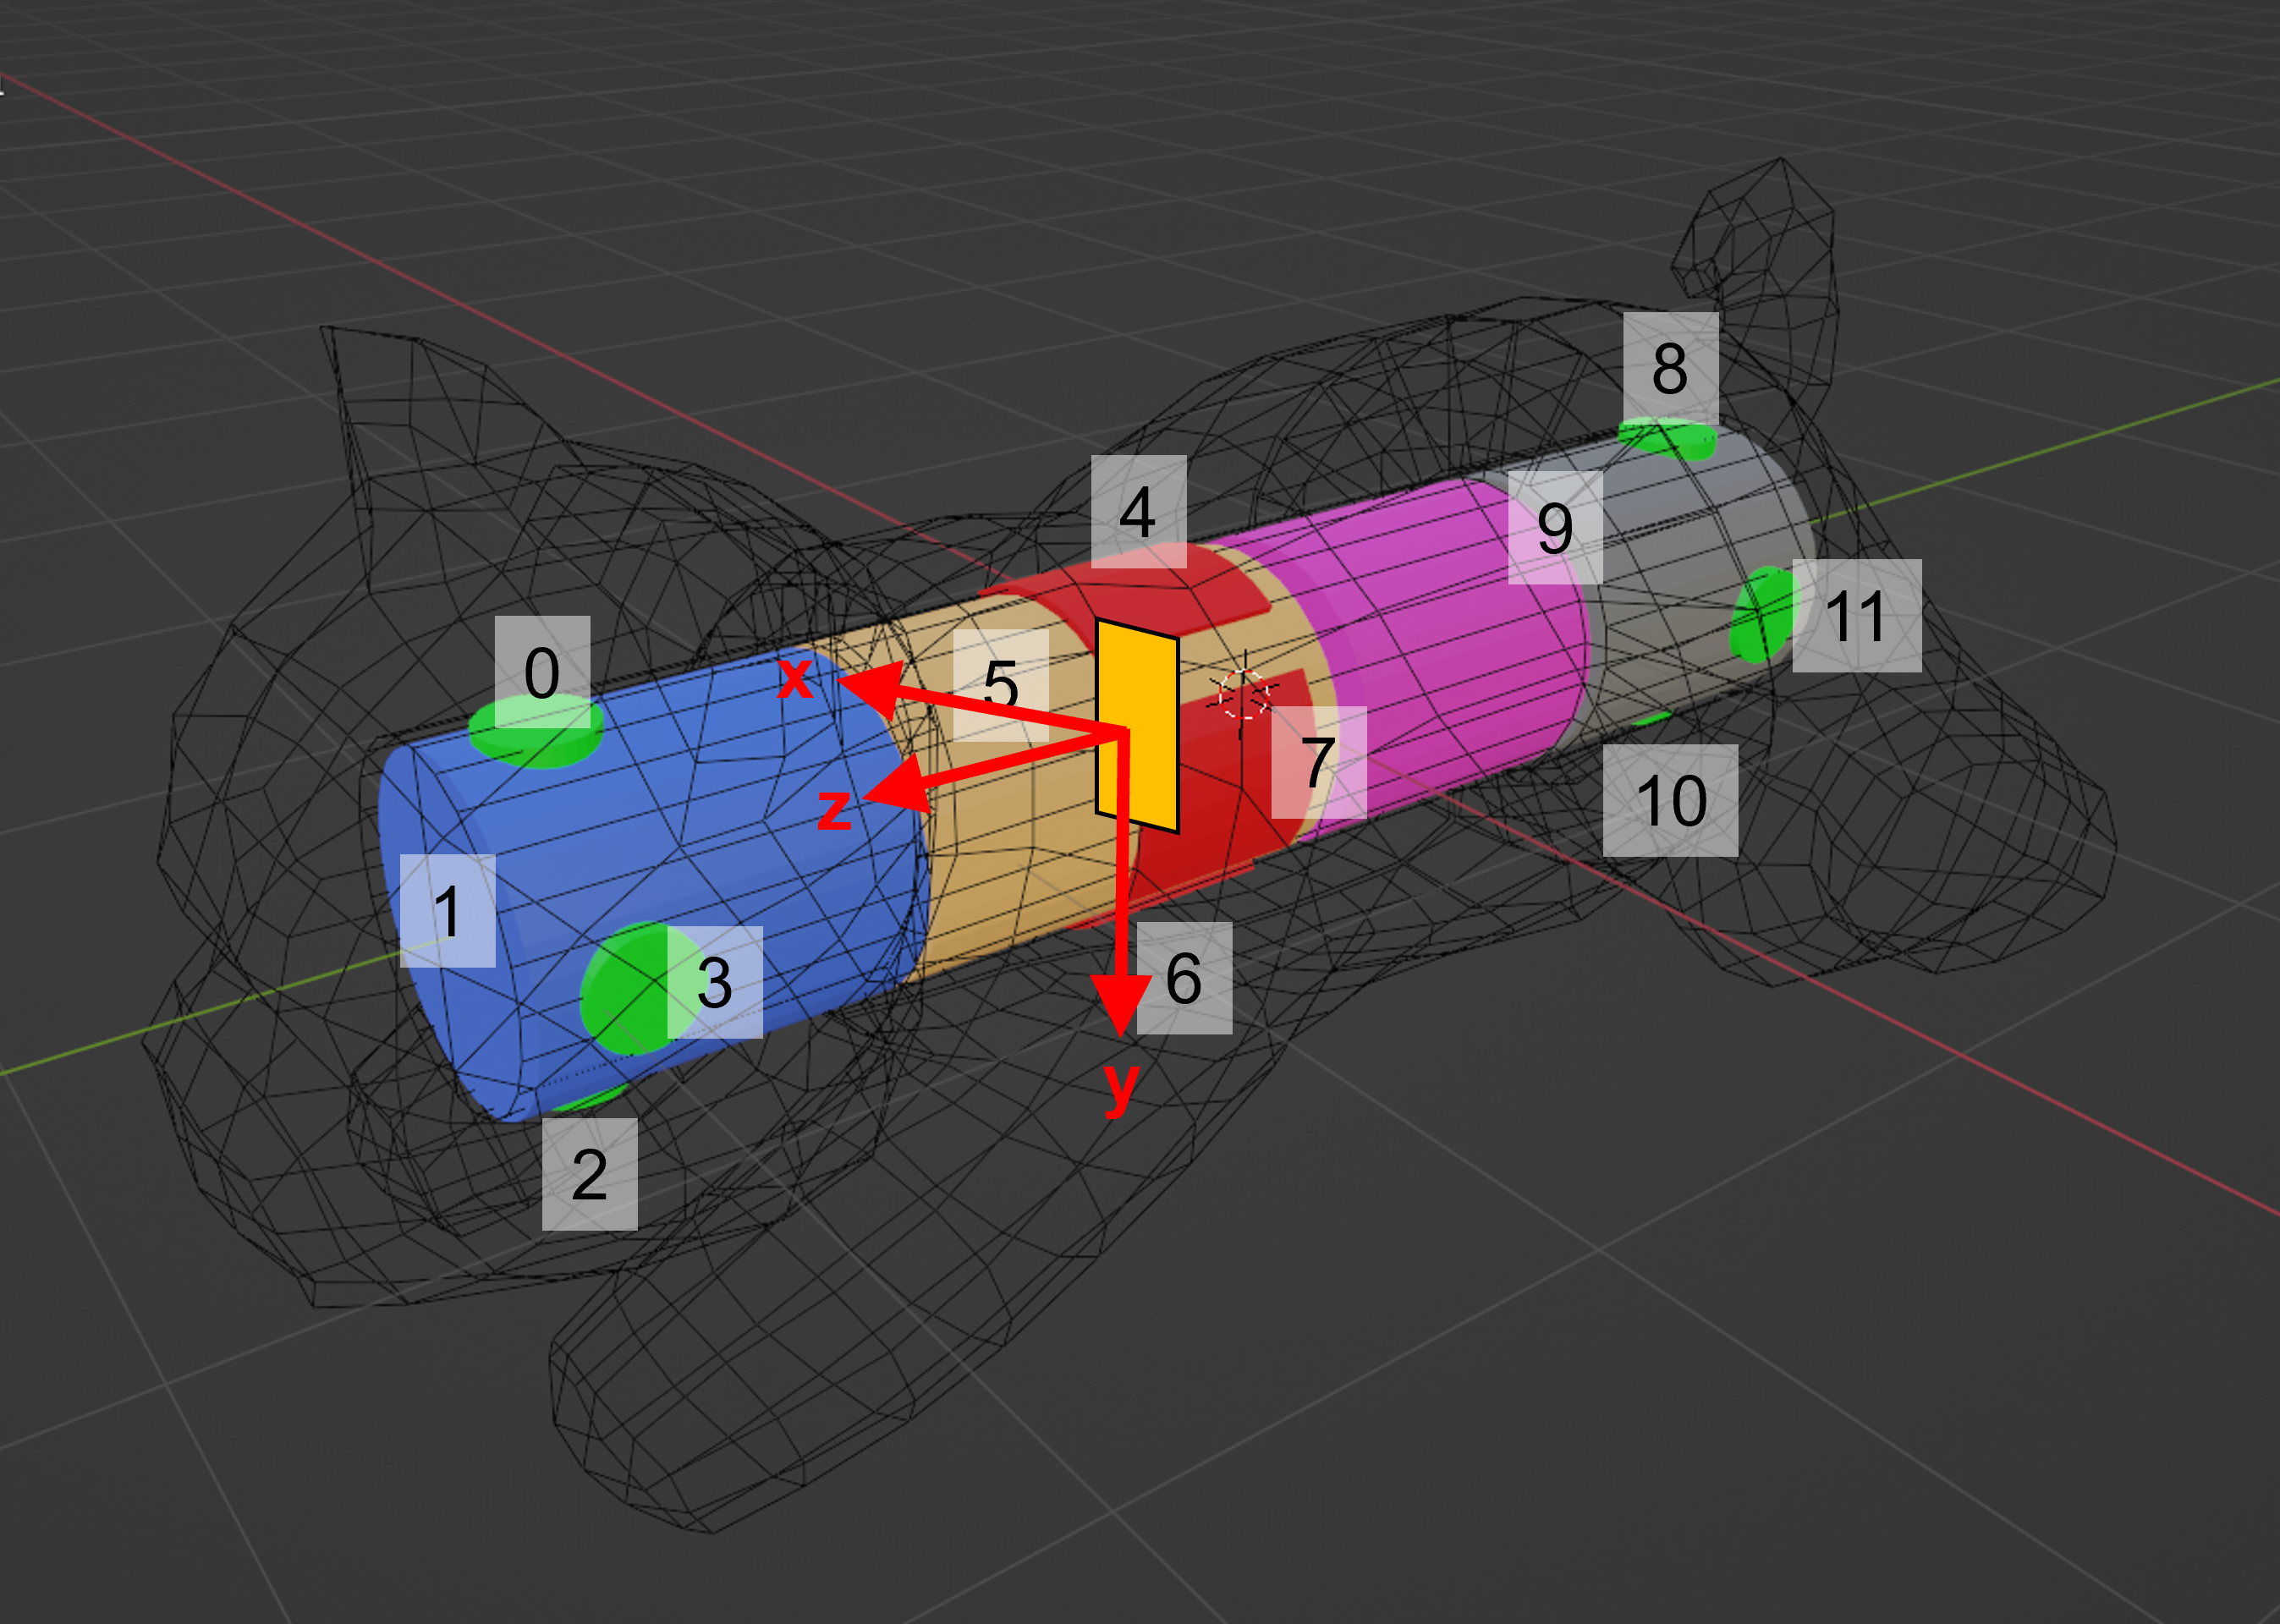
\includegraphics[keepaspectratio,width=6cm,clip]{images/mohukawa/dog_sensor.png}
    \subcaption{MohuCoreとMohuKawaの配置図}
    \label{fig:mohukawa:blender_02}
  \end{minipage}
  \caption{Blenderによる犬のぬいぐるみのモデリング}
  \label{fig:mohukawa:blender}
\end{figure}

\begin{figure}[htbp]
  \centering
  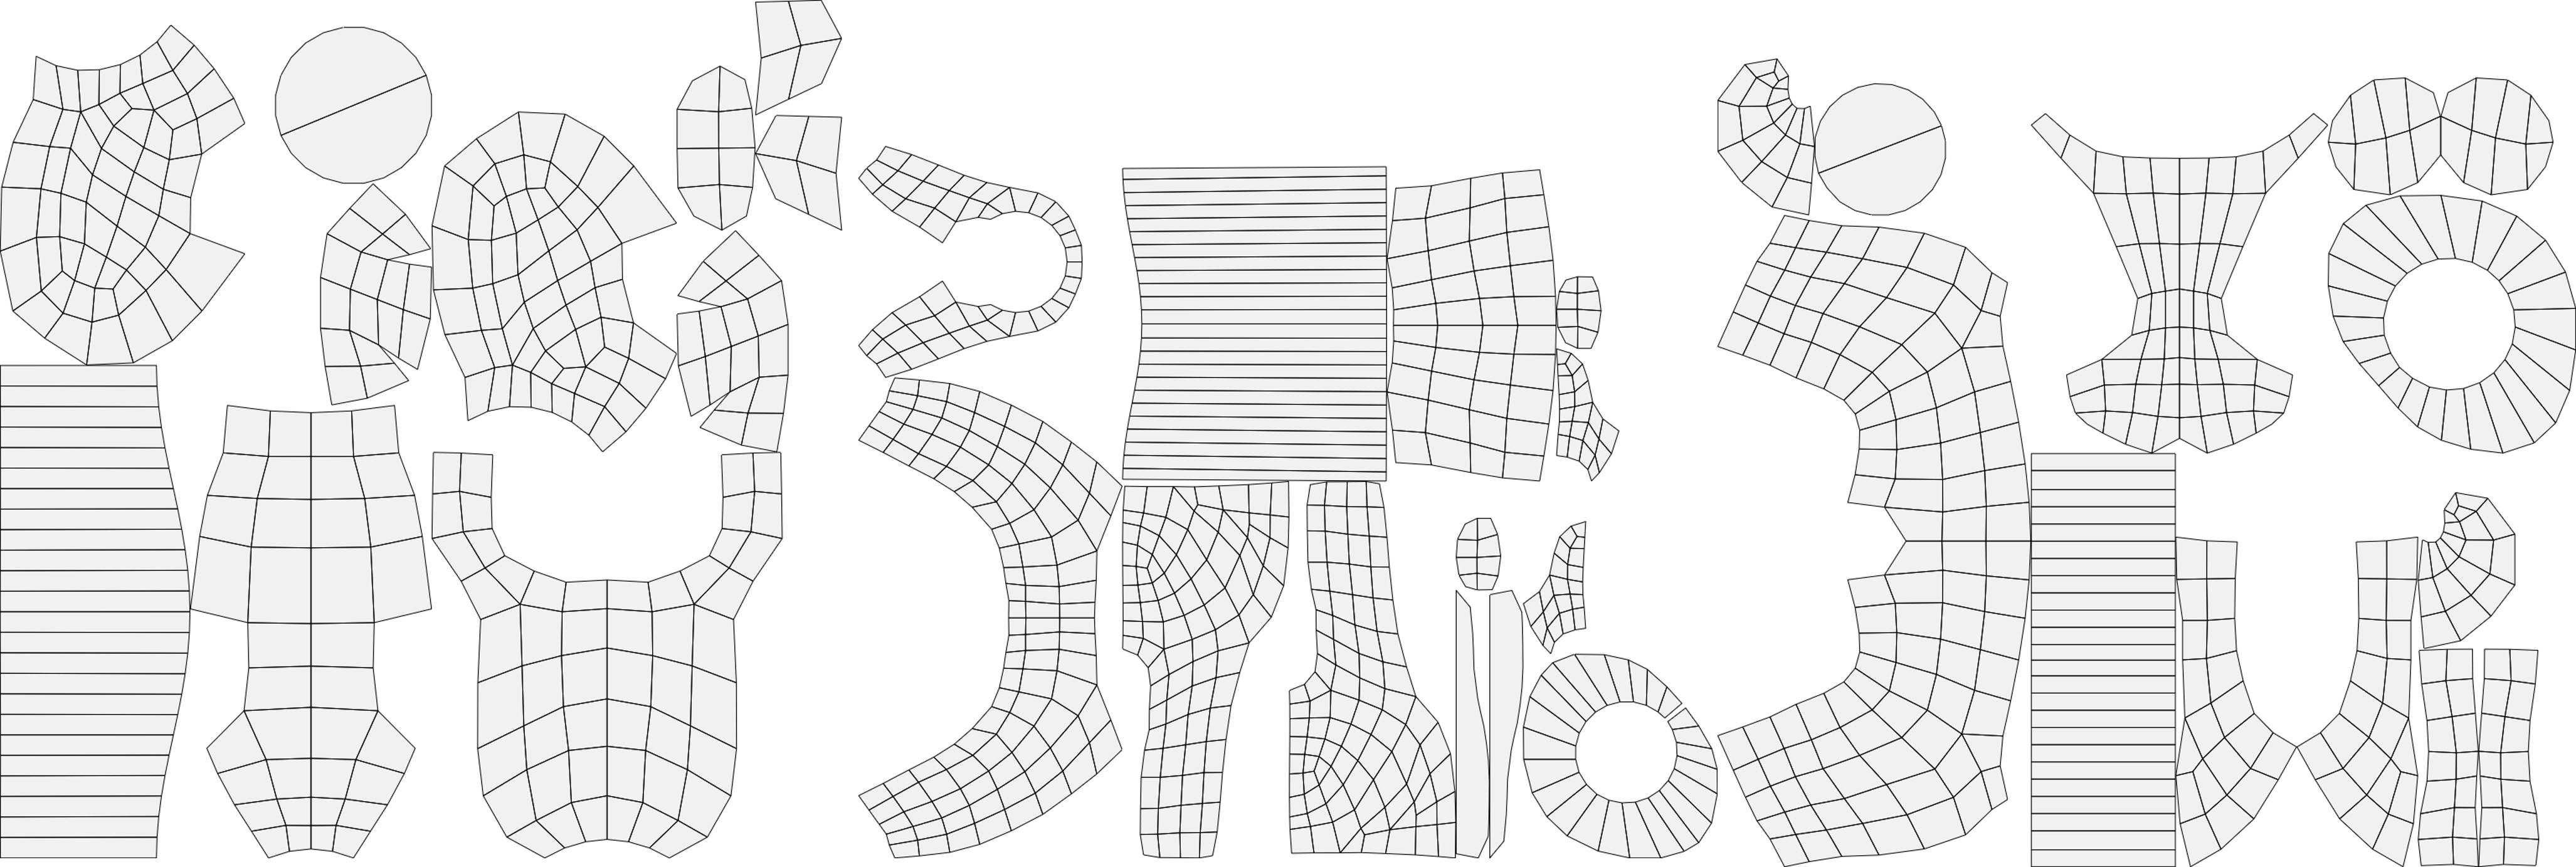
\includegraphics[width=12cm]{images/mohukawa/uv.png}
  \caption{UV展開機能を用いて作成したぬいぐるみの型紙}
  \label{fig:mohukawa:uv}
\end{figure}

\begin{figure}[htbp]
  \centering
  \begin{minipage}[c]{0.48\linewidth}
    \centering
    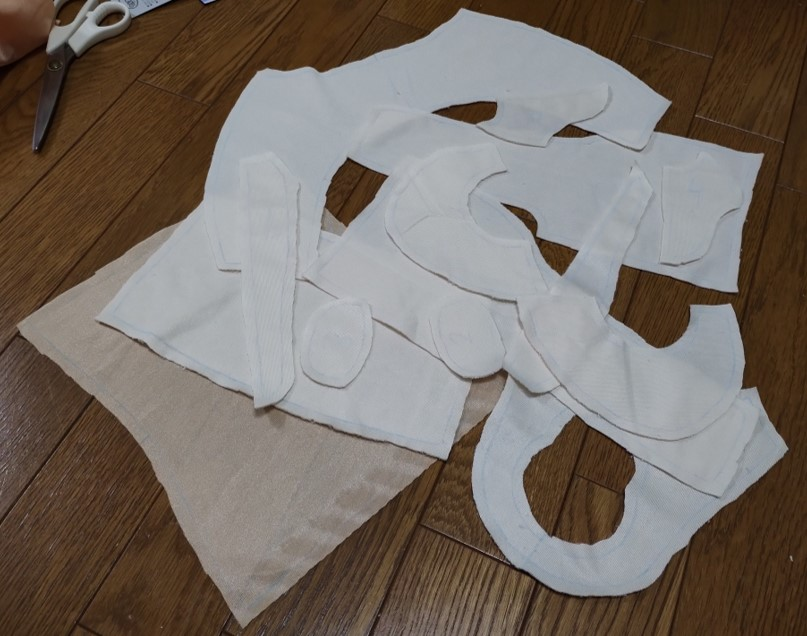
\includegraphics[keepaspectratio,width=4cm,clip]{images/mohukawa/saw_01.jpg}
    \subcaption{生地の裁断}
  \end{minipage}
  \begin{minipage}[c]{0.48\linewidth}
    \centering
    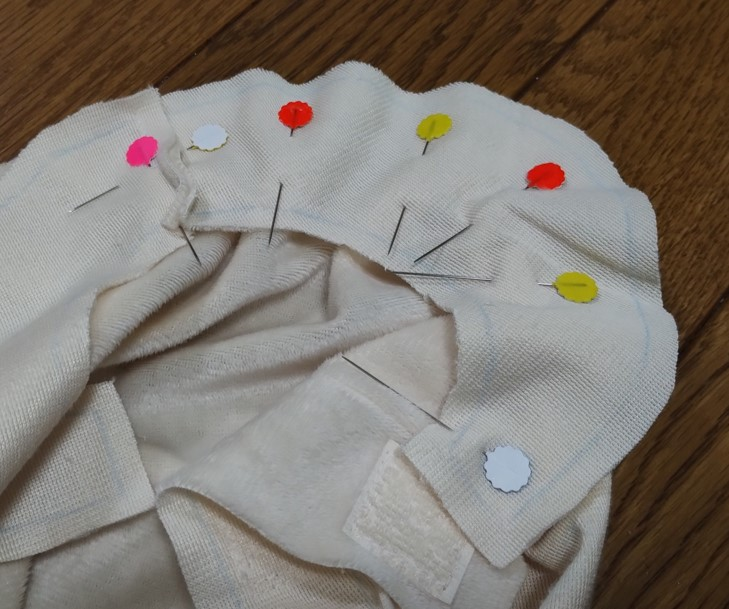
\includegraphics[keepaspectratio,width=4cm,clip]{images/mohukawa/saw_02.jpg}
    \subcaption{生地の縫製}
  \end{minipage} \\
  \begin{minipage}[c]{0.48\linewidth}
    \centering
    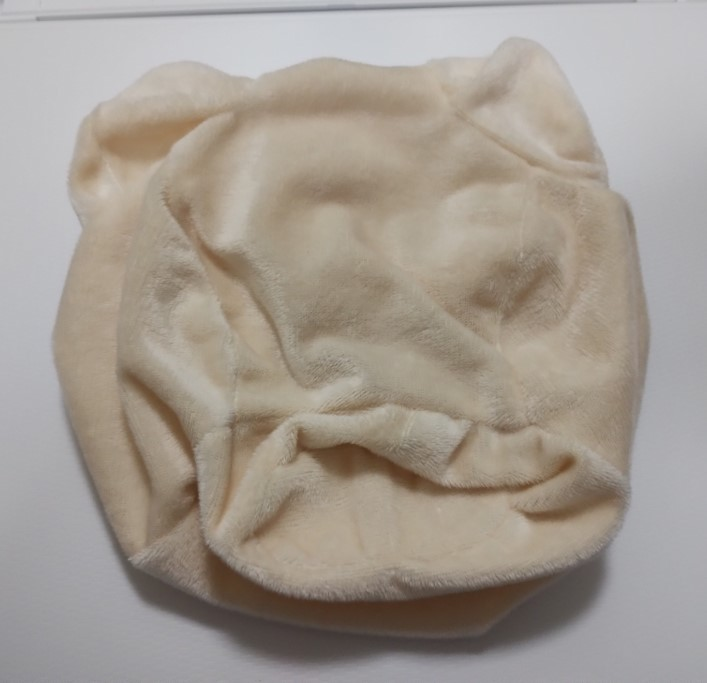
\includegraphics[keepaspectratio,width=4cm,clip]{images/mohukawa/saw_03.jpg}
    \subcaption{犬の頭部(前)}
  \end{minipage}
  \begin{minipage}[c]{0.48\linewidth}
    \centering
    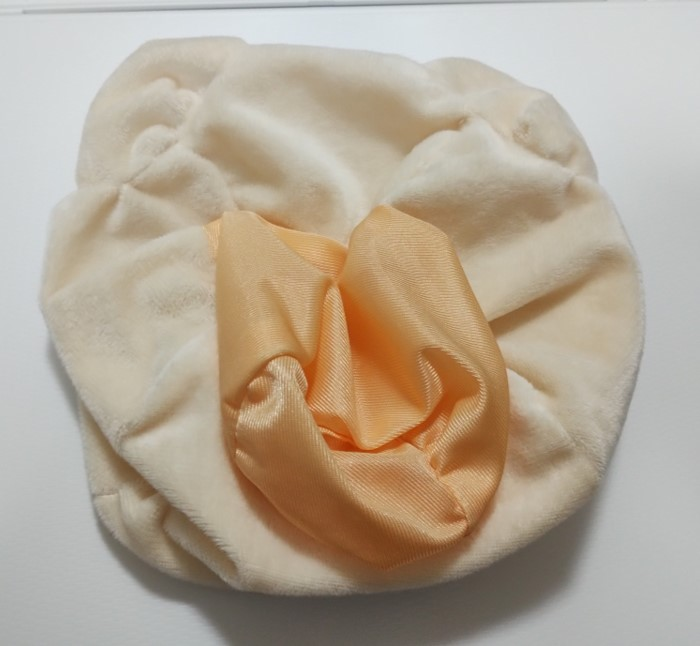
\includegraphics[keepaspectratio,width=4cm,clip]{images/mohukawa/saw_04.jpg}
    \subcaption{犬の頭部(後)}
  \end{minipage}
  \caption{犬のぬいぐるみの縫製の様子}
  \label{fig:mohukawa:saw}
\end{figure}

\begin{figure}[htbp]
  \centering
  \begin{minipage}[c]{0.48\linewidth}
    \centering
    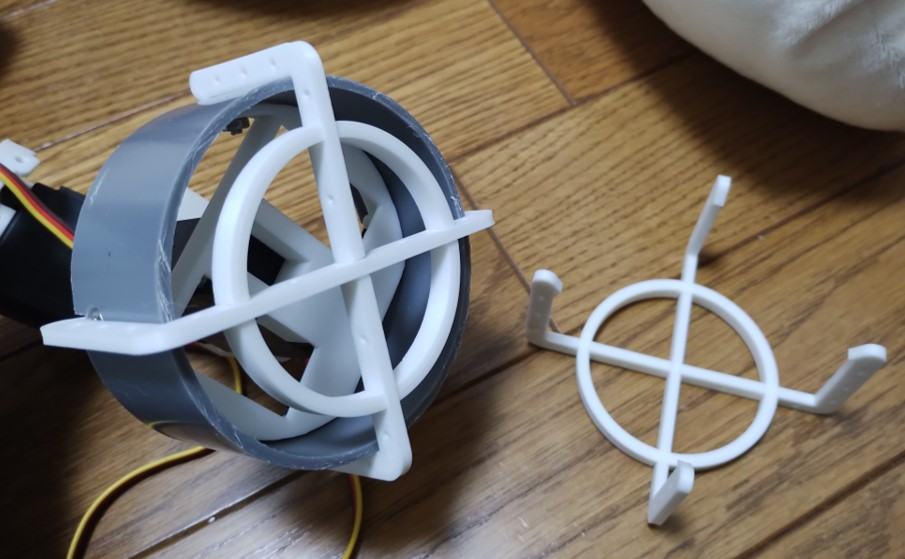
\includegraphics[keepaspectratio,width=4cm,clip]{images/mohukawa/joint_01.jpg}
    \subcaption{3Dプリンタで製作したジョイント}
  \end{minipage}
  \begin{minipage}[c]{0.48\linewidth}
    \centering
    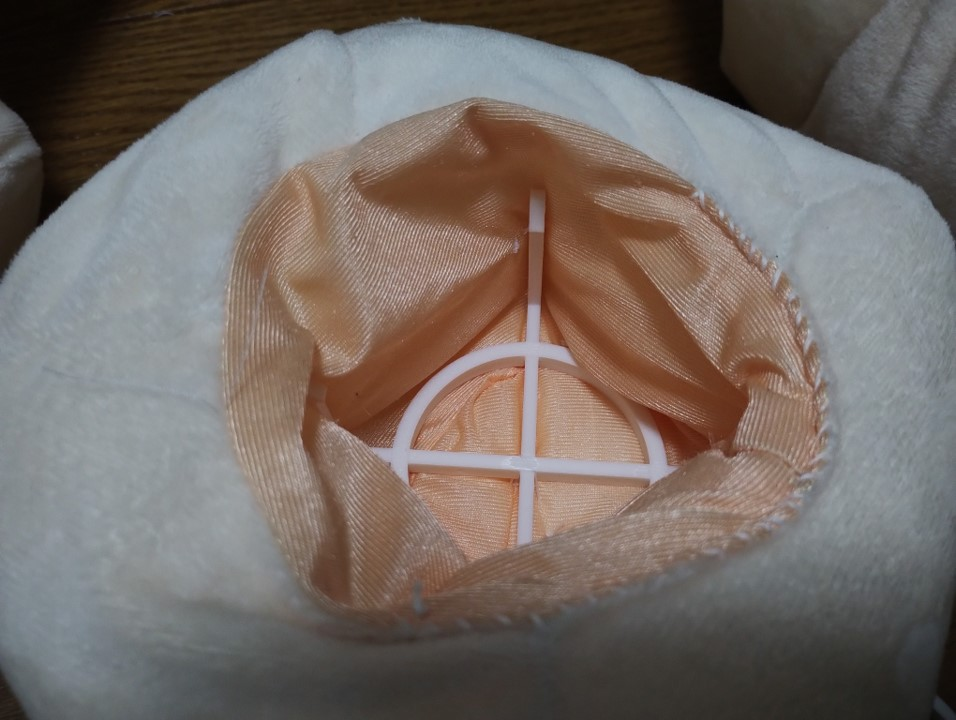
\includegraphics[keepaspectratio,width=4cm,clip]{images/mohukawa/joint_02.jpg}
    \subcaption{ジョイントの埋め込み}
  \end{minipage}
  \caption{犬のぬいぐるみへのジョイントの取り付け}
  \label{fig:mohukawa:joint}
\end{figure}

\begin{figure}[htbp]
  \centering
  \begin{minipage}[c]{0.64\linewidth}
    \centering
    \includegraphics[keepaspectratio,width=8cm,clip]{images/mohukawa/dog_parts.png}
    \subcaption{犬型のぬいぐるみの各パーツ(頭・胴・腰)}
  \end{minipage}
  \begin{minipage}[c]{0.32\linewidth}
    \centering
    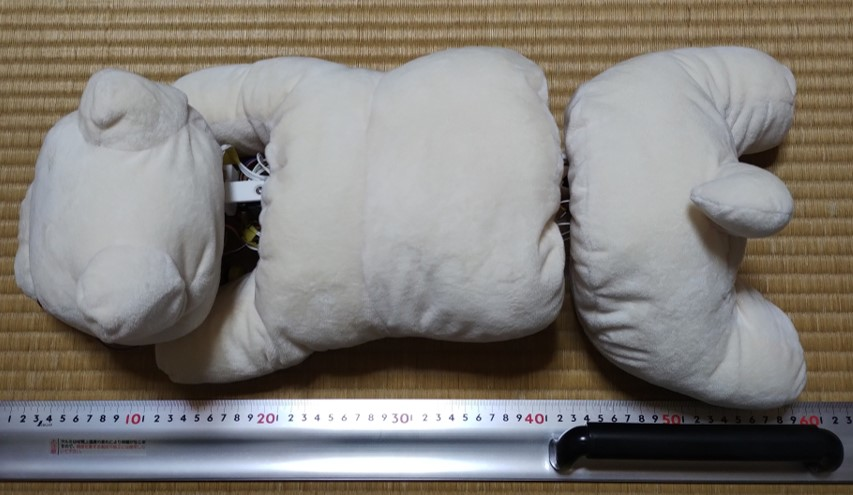
\includegraphics[keepaspectratio,width=4cm,clip]{images/mohukawa/dog.jpg}
    \subcaption{犬型のぬいぐるみ}
  \end{minipage}
  \caption{完全新規設計のMohuKawa}
  \label{fig:mohukawa:dog}
\end{figure}

\subsubsection{市販品を改造して製作されたMohuKawa}
市販のぬいぐるみを改造したMohuKawaでは、全長50cmほどの比較的大きめのぬいぐるみを用いた。
そして、一旦ぬいぐるみを切り開いて綿を取り出した後にMohuCoreを収めるための布を縫い付けた。
最後に、犬の時と同様のジョイントを取り付けてから綿を詰め直してぬいぐるみとした(\figref{fig:mohukawa:anago_making})。
同様にして、人型・パンダ型のぬいぐるみにも加工を施した(\figref{fig:mohukawa:funio_anago_panda})。
\begin{figure}[htbp]
  \centering
  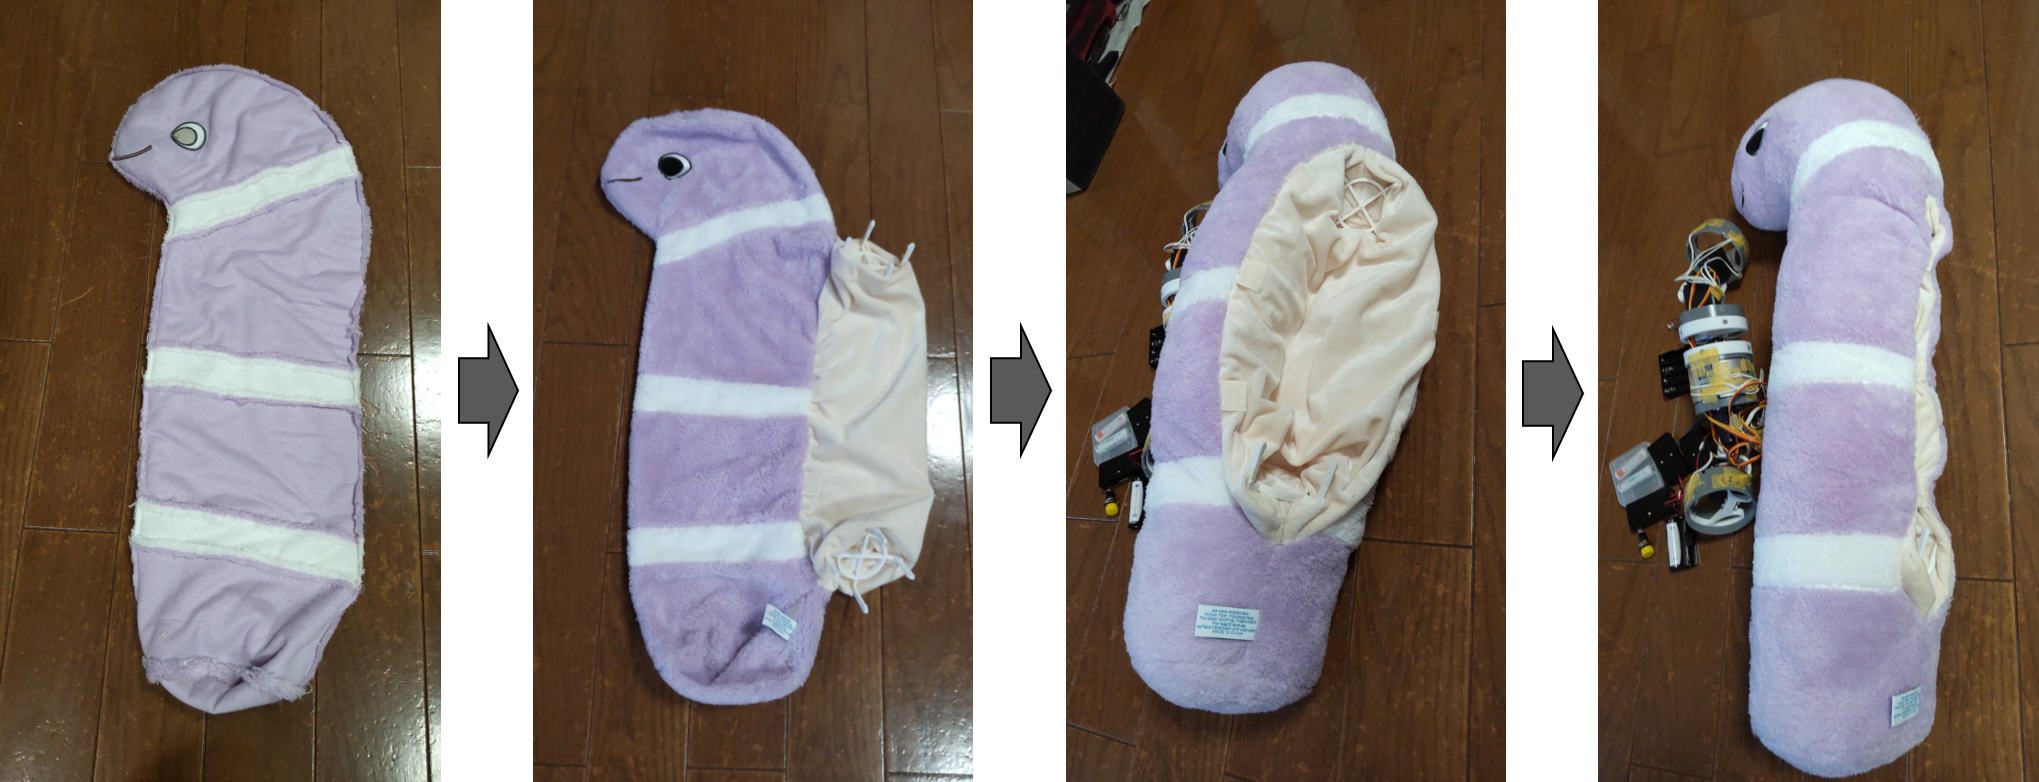
\includegraphics[width=12cm]{images/mohukawa/anago_making.png}
  \caption{市販のアナゴ型のぬいぐるみの加工工程}
  \label{fig:mohukawa:anago_making}
\end{figure}

\begin{figure}[htbp]
  \centering
  \begin{minipage}[c]{0.32\linewidth}
    \centering
    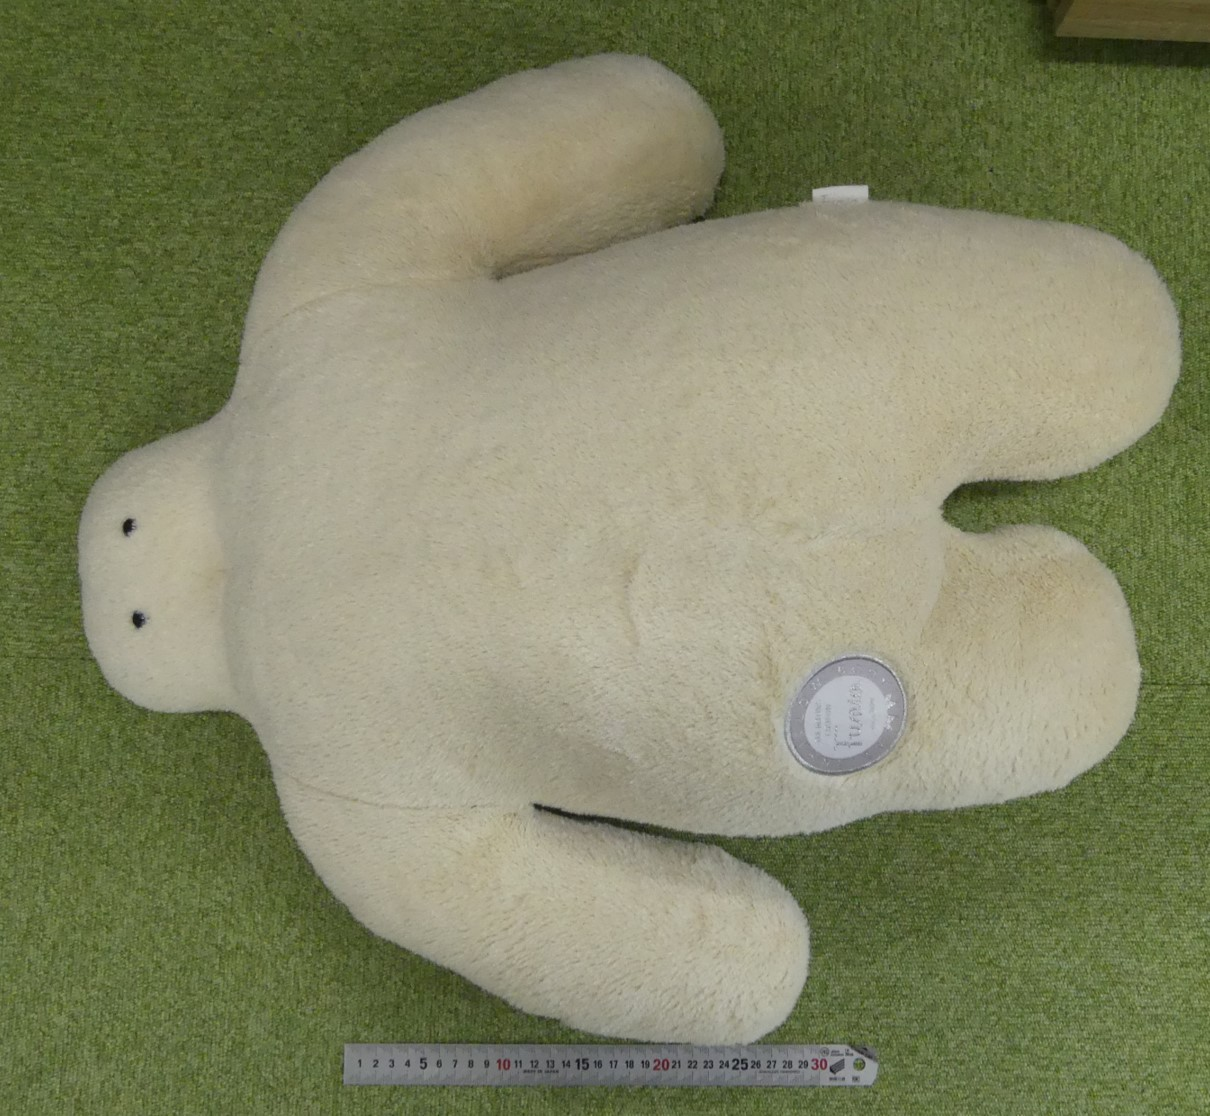
\includegraphics[keepaspectratio,width=4cm,clip]{images/mohukawa/funio.jpg}
    \subcaption{人型のぬいぐるみ}
  \end{minipage}
  \begin{minipage}[c]{0.32\linewidth}
    \centering
    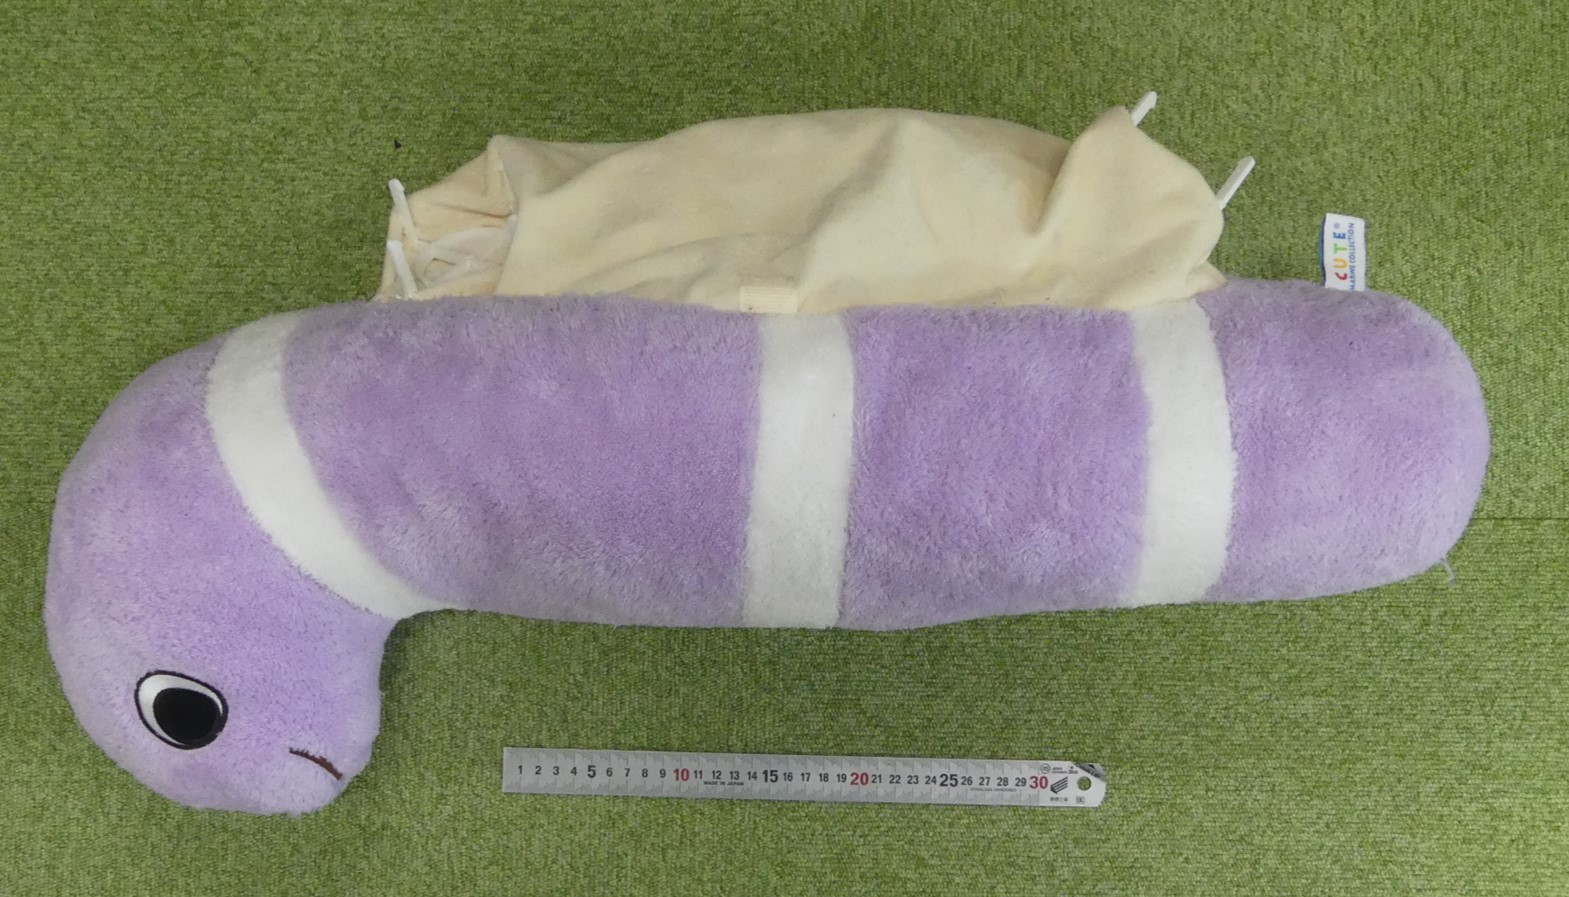
\includegraphics[keepaspectratio,width=4cm,clip]{images/mohukawa/anago.jpg}
    \subcaption{アナゴ型のぬいぐるみ}
  \end{minipage}
  \begin{minipage}[c]{0.32\linewidth}
    \centering
    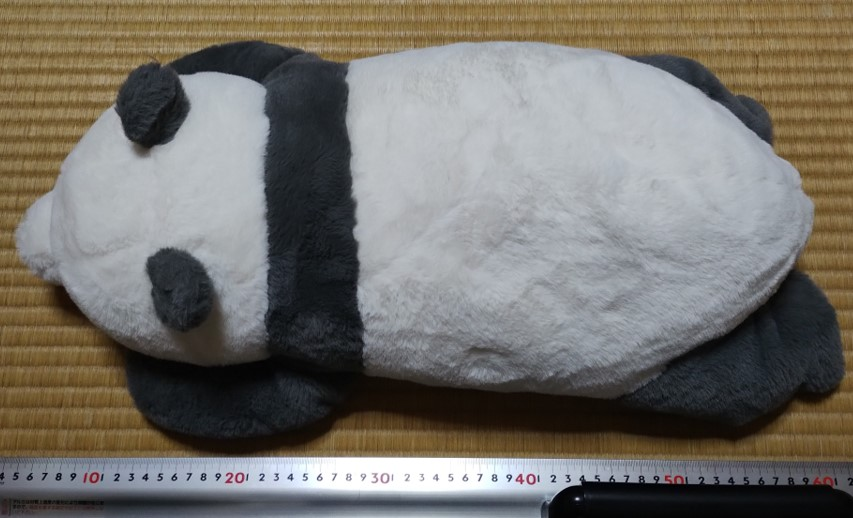
\includegraphics[keepaspectratio,width=4cm,clip]{images/mohukawa/panda.jpg}
    \subcaption{パンダ型のぬいぐるみ}
  \end{minipage}
  \caption{市販品を改造して製作されたMohuKawa}
  \label{fig:mohukawa:funio_anago_panda}
\end{figure}


\subsection{骨格MohuCoreと毛皮MohuKawaの組み立て}
MohuCoreとMohuKawaの組み立てを実際に行い、組み立ての難易度を検証した。
犬型のぬいぐるみでは、まずMohuCoreに犬の頭と腰を取り付け、最後に胴を巻き付けてマジックテープで止めて完成となる(\figref{fig:mohutics:embed_dog})。
人型・アナゴ型・パンダ型のぬいぐるみでは、ぬいぐるみにMohuCoreを差し込んでから、MohuCoreの両端にぬいぐるみのジョイントを取り付け、最後にマジックテープで止めて完成となる(\figref{fig:mohutics:embed_funio})。
いずれのぬいぐるみについても、何度か練習すると1分30秒程度でぬいぐるみの取り付けが可能であった。
つまり、Mohuticsを採用するぬいぐるみロボットでは、ユーザはMohuCoreと自分の好きなMohuKawaを組み合わせることで、ものの数分で自分のお気に入りの見た目のぬいぐるみロボットを手に入れられることになる。
既存のロボットでは見た目の種類が限られてくる一方で、Mohuticsでは多様な姿のロボットを簡単に作ることが可能だと確認できた。

\begin{figure}[htbp]
  \centering
  \begin{minipage}[c]{\linewidth}
    \centering
    \includegraphics[keepaspectratio,width=12cm,clip]{images/mohutics/embed_dog_head.png}
    \subcaption{頭の取り付け}
  \end{minipage} \\
  \begin{minipage}[c]{\linewidth}
    \centering
    \includegraphics[keepaspectratio,width=12cm,clip]{images/mohutics/embed_dog_body.png}
    \subcaption{胴の取り付け}
  \end{minipage}
  \caption{犬型のぬいぐるみロボットの組み立て}
  \label{fig:mohutics:embed_dog}
\end{figure}

\begin{figure}[htbp]
  \centering
  \includegraphics[width=12cm]{images/mohutics/embed_funio.png}
  \caption{人型のぬいぐるみロボットの組み立て}
  \label{fig:mohutics:embed_funio}
\end{figure}

\subsection{知能MohuAIの開発}

ロボット開発では、ハードウェアとの入出力を直接扱う低レイヤー層やロボットの動作計画等のハードウェアを直接触れない高いレイヤーの層を異なるパッケージにまとめるなど、ハードウェア等への依存度に応じてプログラムを階層化させることが一般的である。
Mohuticsではロボットの電気的・機械的要素を含む骨格は共通化させるため、ぬいぐるみロボットの種類にかかわらず必要なハードウェア関連のソースコードは使いまわせる。
開発ではソースコードをぬいぐるみの種類や盛り込む機能に応じて共通化できる部分とそうでない部分に分割し、開発を進めた。

ハードウェアに近い部分としては、姿勢センサの値を読み出すライブラリの実装(\figref{fig:i2c_wave})やWi-Fiを経由してぬいぐるみロボットに必要なプログラムをダウンロードする機能等を実装した。
また、感圧センサの値に応じてぬいぐるみがユーザの加えた力に抗うような動きを組み込んだ。

\begin{figure}[htbp]
  \centering
  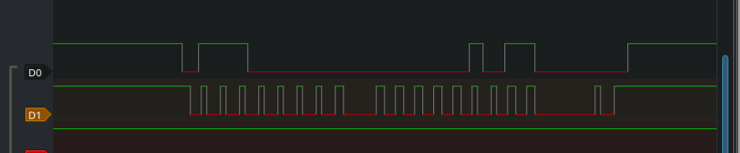
\includegraphics[width=8cm]{images/mohutics/i2c_wave.png}
  \caption{姿勢センサの信号波形の確認}
  \label{fig:i2c_wave}
\end{figure}

(\figref{fig:mohutics:home})に、ぬいぐるみロボットを生活空間に置いた様子を示す。
もともとぬいぐるみであるため、無機的な質感がなく家の中に置いても違和感が少ない。
また、プログラムによっては自発的に動き出すこともあるため、あたかもぬいぐるみが生きているかのような雰囲気が醸し出される。

\begin{figure}[htbp]
  \centering
  \begin{minipage}[c]{0.24\linewidth}
    \centering
    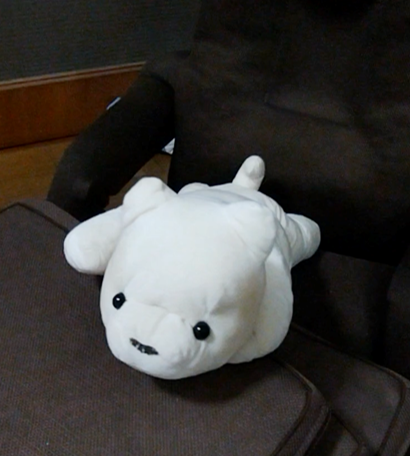
\includegraphics[keepaspectratio,width=3cm,clip]{images/mohutics/dog.png}
    \subcaption{犬型のぬいぐるみ}
  \end{minipage}
  \begin{minipage}[c]{0.24\linewidth}
    \centering
    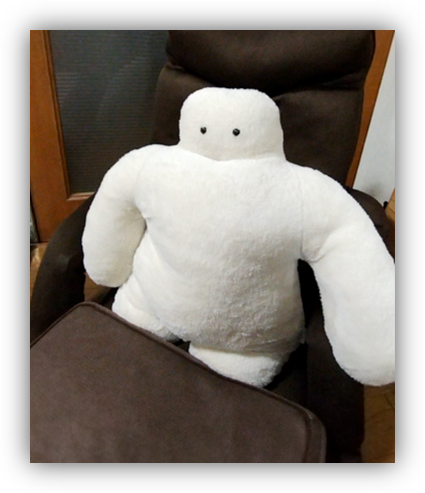
\includegraphics[keepaspectratio,width=3cm,clip]{images/mohutics/funio.png}
    \subcaption{人型のぬいぐるみ}
  \end{minipage}
  \begin{minipage}[c]{0.24\linewidth}
    \centering
    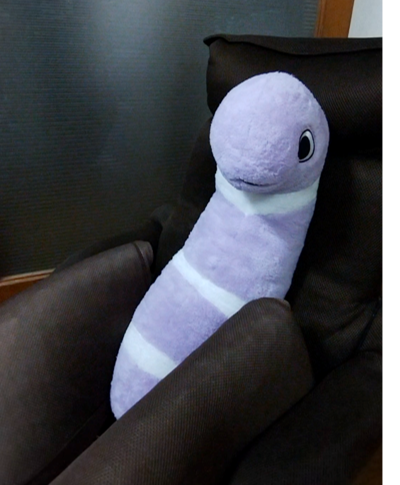
\includegraphics[keepaspectratio,width=3cm,clip]{images/mohutics/anago.png}
    \subcaption{アナゴ型のぬいぐるみ}
  \end{minipage}
  \begin{minipage}[c]{0.24\linewidth}
    \centering
    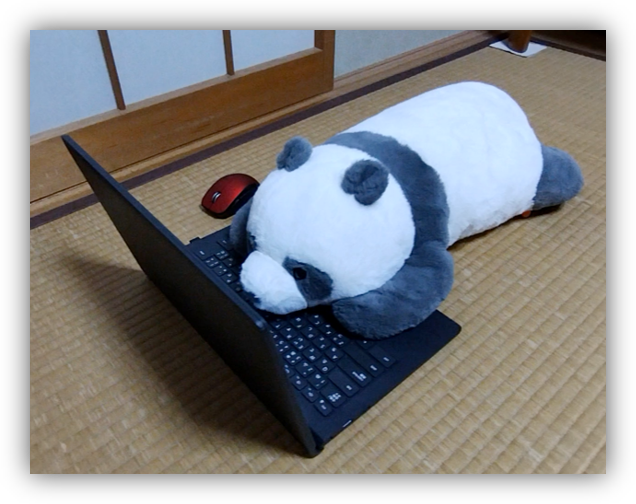
\includegraphics[keepaspectratio,width=3cm,clip]{images/mohutics/panda.png}
    \subcaption{パンダ型のぬいぐるみ}
  \end{minipage}
  \caption{生活空間に溶け込むぬいぐるみロボット}
  \label{fig:mohutics:home}
\end{figure}

また、ぬいぐるみロボットと人とのインタラクションに関して、ぬいぐるみの種類が異なる場合に人の触れ合い方が変わるのかを検証した。
そのために、機械学習を用いてぬいぐるみロボットに対する人間のインタラクション方法の分類を行った。
この実装を行った時点ではMohuCoreのCPUにESP32を用いており、計算能力の不足が懸念されたため有線で外部のパソコンと接続している(\figref{fig:learning})。
そして、姿勢センサと感圧センサの値をパソコンに送信し、そのセンサの時系列情報から、現在人がどの種類のぬいぐるみと触れ合っているかの推定を行わせた。
ぬいぐるみには犬型・人型・アナゴ型を用い、事前にユーザにそれらのぬいぐるみと抱っこしてもらうなどして訓練データを用意した。
そして、訓練やテストにはPyTorchによる単層または2層のニューラルネットと教師あり学習を利用した。

検証では、ユーザにぬいぐるみを抱いてもらうなどして抱き方の時系列情報とぬいぐるみの種類の対応をとった訓練データを用意した。
そして、テストデータとして用意したセンサの情報から正しいぬいぐるみの種類を3種類の中から当てられるかを検証した。
結果としては、特定の個人内では抱き方などから9割ほどの正答率でぬいぐるみの種類を当てられた。

この検証はぬいぐるみロボットのセンサと機械学習の組み合わせからどの程度有用な情報が得られるかを調べるために行われたため、この実装自体がそのままぬいぐるみロボットに適用できるわけではない。
しかし、さらなる改良を加えることで、抱き方の傾向からぬいぐるみロボットが今自分を触っている相手が持ち主かどうかを判定し、それによって振る舞いを切り替えるといった機能は実現可能だと考えられる。


\begin{figure}[htbp]
  \centering
  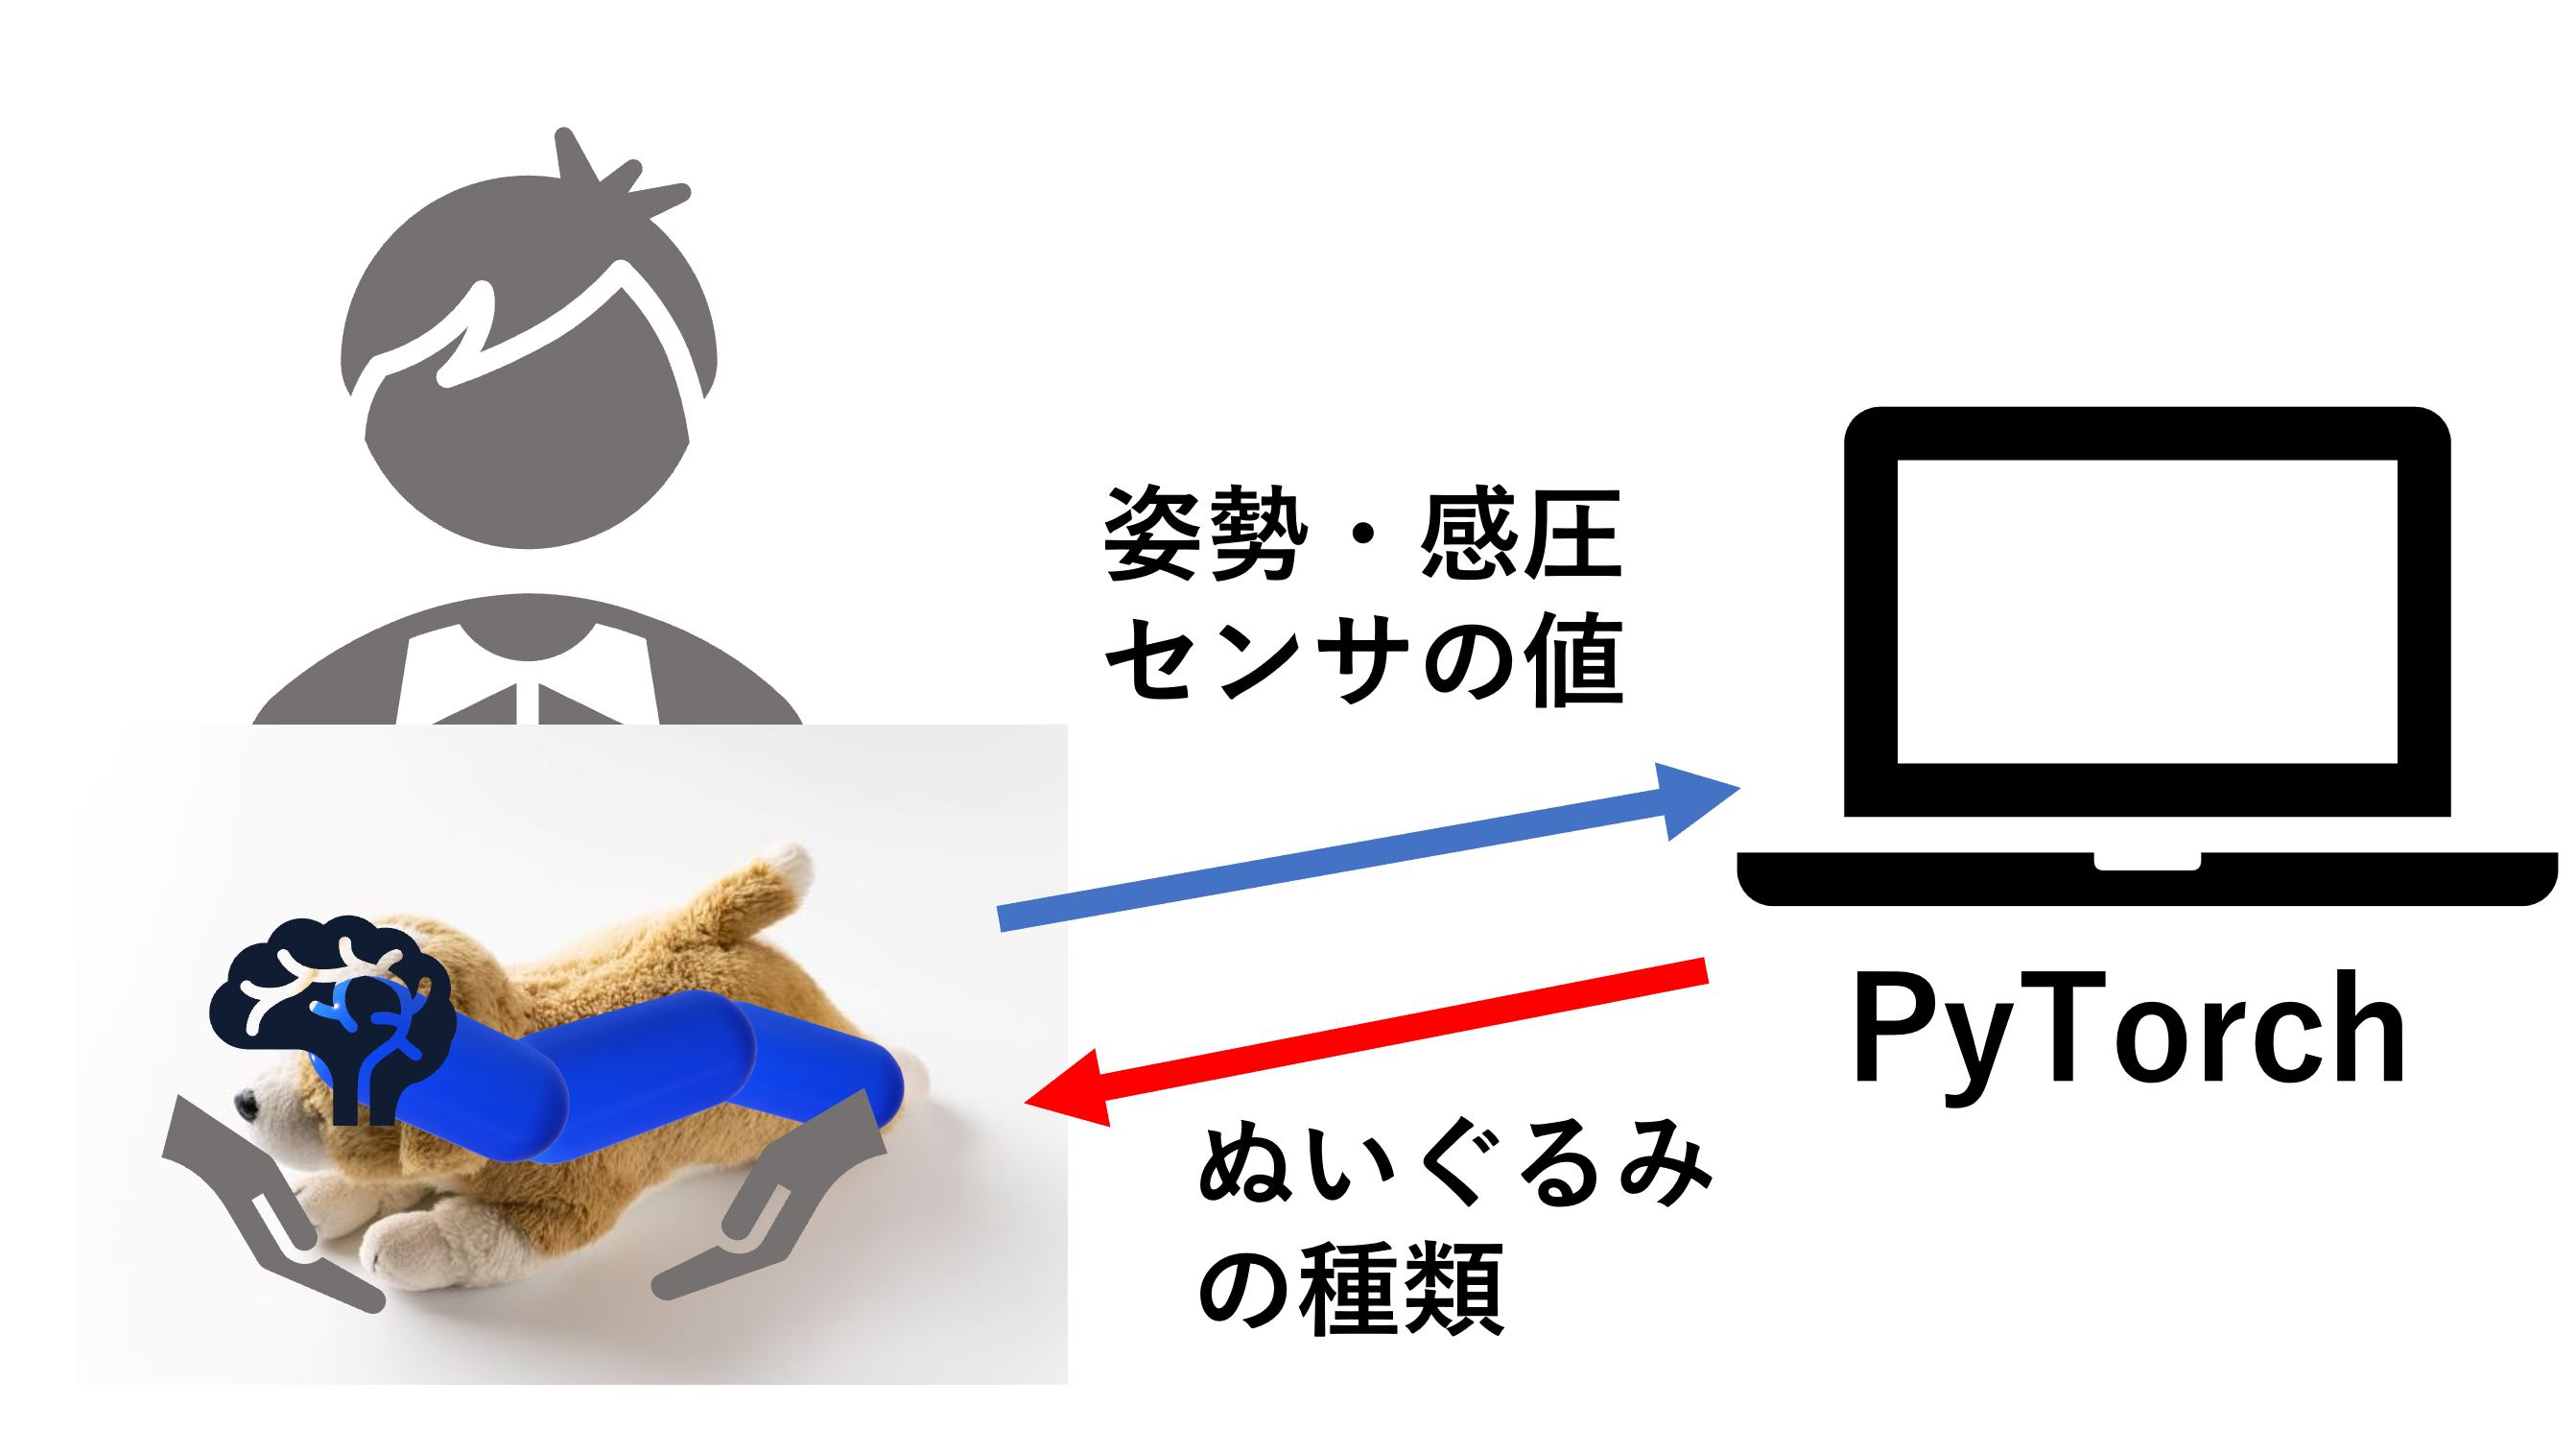
\includegraphics[width=8cm]{images/mohutics/learning.png}
  \caption{外部PCを利用したぬいぐるみロボットに対する人のインタラクション方法の分類}
  \label{fig:learning}
\end{figure}

\begin{figure}[htbp]
  \centering
  \begin{minipage}[c]{0.96\linewidth}
    \centering
    \includegraphics[keepaspectratio,width=12cm,clip]{images/mohutics/dog_interaction_01.png}
    \subcaption{犬型のぬいぐるみ}
  \end{minipage} \\
  \begin{minipage}[c]{0.96\linewidth}
    \centering
    \includegraphics[keepaspectratio,width=4cm,clip]{images/mohutics/funio_interaction_01.png}
    \subcaption{人型のぬいぐるみ}
  \end{minipage}
  \caption{人とぬいぐるみロボットのインタラクション傾向の検証の様子}
  \label{fig:mohutics:interaction}
\end{figure}



\subsection{ユーザ評価}
ぬいぐるみロボットと触れ合ったユーザから、実際に触ってみた時の感想の聞き取りを行った。

ある20代男性からは、動かないぬいぐるみをただ抱くのではなく、抱いているときにぬいぐるみが自ら動いてくれると落とさないように無意識的に体を動かすので自然に触れ合えるといった意見があった。
また、ぬいぐるみは抱き心地が良いように作られているため、触れ合う上で相手の目やしぐさをずっと見つめずとも触覚だけでインタラクションが完結する。
よって、ぬいぐるみロボットであれば長時間使用しても疲れにくそうだとも話していた。

一方で、これまでの人生でほとんどぬいぐるみと接した経験のない男性からは、ぬいぐるみとどう触れ合えばよいのかわからないという意見があった。
ぬいぐるみロボットが万人受けする分野でないとしても、ぬいぐるみロボットの魅力を伝えたりこちらが新たな魅力に気づいたりするためにも、今後も広く聞き取りを続けることが重要だと考える。

さらに、本事業の成果報告会において、同期のクリエータや未踏事業のPM・OB・OGをはじめとした多くの方々にぬいぐるみロボットと触れ合っていただいた。
多くの方に共通していた感想として、もぞもぞと動くぬいぐるみを抱きかかえるだけで一定の安心感や癒やしを得られるという点がある。
たとえぬいぐるみの毛皮が分厚く動いている様子が外からわかりづらくとも、抱きかかえれば確かに腕の中でぬいぐるみが動いていることがわかる。
プロジェクト開始時は筆者はぬいぐるみロボットをいかに愛らしく動かすかを重視していたが、稲見PMからはむしろぬいぐるみロボットと人とのインタラクションに注目することを勧められた。
この度の成果報告会においてさまざまな年代の方々の感想を聞くことで、人とぬいぐるみロボットが直接触れ合う過程にこそペットでも無機質なロボットでもない、ぬいぐるみロボットの本当の価値があると確信した。

他にも、成果報告会ではぬいぐるみロボットとユーザとの距離感や関係性を問う意見もあった。
ぬいぐるみロボットではぬいぐるみ側から人に声を出すなど働きかけることもできるし、逆に人から働きかけがあった場合にのみぬいぐるみが応答するというコミュニケーション様式にもできる。
筆者は現在、基本的には人から働かけがあった場合にぬいぐるみとのコミュニケーションが始まるといった距離感が、ぬいぐるみの良さをうまく引き出せるのではないかと考えている。
しかし、筆者の一人暮らしの経験上、孤独に陥ってしまうと、たとえ大切なぬいぐるみであっても自ら働きかけることが非常に億劫になる場合があると感じる。
よって、カメラを取り付けるなどして、ぬいぐるみとたまたま目が合うなど、ユーザの無意識的なしぐさをぬいぐるみロボットが感知し持ち主に積極的に働きかけることも少なからず必要であろうと考える。

このように、実際にユーザの声を聞くことで本プロジェクトの魅力や進むべき方向性を再認識することができた。

\section{開発成果の特徴}
本プロジェクトでは、様々な種類のぬいぐるみを効率的にロボット化するぬいぐるみロボットシステムMohuticsを提案し、実際にぬいぐるみ部分の換装が可能なロボットシステムのハードウェアやソフトウェアを製作することで、その基盤を整えた。
特に、ぬいぐるみ部分の取り付けは工具を使わずに1分30秒ほどで行えるため、自分の好きな見た目のロボットを迎えるためのハードルを大きく下げたといえる。

さらに、ぬいぐるみロボットと機械学習を組み合わせ、人のインタラクションをぬいぐるみロボットが認識する一例を示した。


\section{今後の課題、展望}\label{sec:challenges}
本プロジェクトではシステムの簡素化及び省電力化を意図し、ロボットをESP32という比較的計算能力の低いマイクロコントローラを用いて設計した。
しかし、機械学習のスタンドアロンな実装やクラウドサービス等の連携を踏まえると、Linuxといった高機能なOSを搭載可能なシングルボードコンピュータを用いた方が発展性に富む。

本プロジェクト後半では、Raspberry Pi Zero 2Wという組み込み開発向けLinuxボードを使用し、計算能力を大幅に向上させた改良型も製作した(\figref{fig:prototype_04})。
この改良型では、サーボモータについても電流制御等が可能で動きも滑らかな高性能なものを搭載し、ぬいぐるみロボットとしての抱き心地を改善している。

\begin{figure}[htbp]
  \centering
  \begin{minipage}[c]{0.48\linewidth}
    \centering
    \includegraphics[keepaspectratio,width=6cm,clip]{images/prototype/prototype_04_01.jpg}
    \subcaption{改良型MohuCore}
  \end{minipage}
  \begin{minipage}[c]{0.48\linewidth}
    \centering
    \includegraphics[keepaspectratio,width=6cm,clip]{images/prototype/prototype_04_02.jpg}
    \subcaption{犬型のぬいぐるみとの組み合わせ}
  \end{minipage}
  \caption{2024年3月現在開発中の改良型MohuCore}
  \label{fig:prototype_04}
\end{figure}

今後、ROS2といった汎用的なロボット開発フレームワークにプログラムコードを移植し、カメラや機械学習、クラウドなどとの連携が容易になる土台を整えてから、ぬいぐるみロボットのさらなる機能強化を進めたいと考えている。

展望としては、本プロジェクトで製作したぬいぐるみロボットシステムの開発を進め、いずれは製品として社会に広めることを目標としている。

まず、開発の大きな目標としては、本プロジェクトのロボットに人工知能分野の技術をさらに盛り込むことが考えられる。
現時点ではロボットが姿勢や触覚センサの情報から機械学習を用いてぬいぐるみの種類を識別する機能が実装されている。
これを発展させていけば、ロボットがユーザ特有のインタラクションのパターンを読み取って持ち主を認識できたりするであろう。

また、近年注目されるXR分野への適用も期待される。
インターネット上の仮想空間で会話を行えるVRChatのようなサービスに自身が抱いているぬいぐるみロボットを持ち込むことや、遠方の家族とぬいぐるみを通して握手や会話といったインタラクションを行うことは2024年3月現在開発中のハードウェアで実現可能だと考えている。

次に、本プロジェクトの社会への普及についても述べる。

ぬいぐるみロボットシステムMohuticsの特徴として、ぬいぐるみロボットに必要なロボットの開発とぬいぐるみの製造という全く異なる技術を、それぞれMohuCoreやMohuKawaなどとして適切に分割した点が挙げられる。
これにより、共通化されたロボット部分のMohuCoreはロボット開発が得意な筆者を中心とした組織が設計・開発し、多くの種類が必要でかつ縫製のノウハウも求められるMohuKawaはぬいぐるみメーカーに製造を委託するといったことが可能になる。
将来的にはMohuKawaを製造する各ぬいぐるみメーカーにMohutics対応を謳うためのライセンスを販売し、その収益をMohuCoreの開発に活用するといったビジネスモデルも考えられよう。

さらに、ロボットのソフトウェア部分のMohuAIはオープンソースにすることが重要だと考えている。
本プロジェクトで開発したMohuticsは、ユーザの多様な好みに寄り添うための開かれたぬいぐるみロボットを目指している。
しかし、ソフトウェアによってロボットに様々な機能を搭載できたとしても、それがあらゆるユーザの需要を満たせるとは限らないし、ユーザが見つけても筆者が気づかなかったぬいぐるみロボットの新たな可能性を見落とすことになりかねない。
よって、ソースコードを公開し意欲のあるユーザにはプログラムを改変する余地を残すことが、ぬいぐるみロボットという発展途上の分野を育む上で重要だと考えている。

さらに、ぬいぐるみロボットは動物と異なり明確な死がないため、その運用は10年や20年といった長期に渡る可能性がある。
電子機器ではしばしば製造メーカーのソフトウェアの保守期間の終了が機器の運用に終わりを告げることがあるが、大手メーカーでもない限り、長期的なサポートをユーザに約束することは難しい。
特にぬいぐるみロボットは人の心に寄り添う愛玩対象であるため、メーカー側の都合でサポートが途切れる事態は避けることが望ましい。
したがって、ソフトウェアをオープンソースとし、Mohuticsが一定の技術を持つ有志の手で保守可能であると明示することが購買に関心のある客の安心感につながり、結果的にぬいぐるみロボットの長期的な発展につながると考えている。


\section{実施計画書内容との相違点}
\subsection{ユーザ評価とぬいぐるみロボットとしてのAIに対する筆者自身の考え}
ぬいぐるみロボットであれば人とのインタラクションを重視すべきというPMの助言を受け、実際にユーザに触ってもらうことに注力した。
プロジェクト初期は筆者自身がぬいぐるみに必要なAIとしての要素を模索している段階であり、実施計画書ではぬいぐるみロボットに実装する知能についての記述は漠然としたものだった。
そこで、ユーザのインタラクションの検証等を通して考え、現在では本プロジェクトで実装すべきぬいぐるみの知能を「ぬいぐるみが人とのインタラクションを通すことで初めて得られる情報を理解する力」としている。

本プロジェクトで行われた人とぬいぐるみロボットとのインタラクションの機械学習による分析は検証方法に改善の余地を残している。
一方で、この検証は、いずれは「ぬいぐるみロボットは人に抱かれることで、その動かし方のパターンなどから自身のぬいぐるみとしての容姿や形状の情報を人から引き出している」という仮説を裏付けていくと考えている。
まだ計算能力の都合で機械学習機能をスタンドアロン化できていないなど改善点は多いが、本プロジェクトを通して自分なりのぬいぐるみロボットにおける知能の在り方を整理できたことは意義が大きかった。

\subsection{ハードウェアの仕様変更}
当初はMohuCoreによって無線通信を使いMohuKawaの種類を自動で認識する機能の実装を検討していた。
しかしこれはPMとのミーティングを通してCPUの種類や入手可能な部品によってハードウェア関連の実装が大きく変わる上にぬいぐるみロボットの本質から外れると判断したため、ぬいぐるみの種類によるプログラムの切り替えは外部のボタン入力を用いたものにとどめている。

MohuCoreのCPUを何度か変更したことに伴って、マイコンの機能の制約から(\figref{fig:mohucore:skeleton})に示すMohuCoreには音声関連の機能が実装されていない。
ただし、現在製作中の改良型(\figref{fig:prototype_04})では音声処理が問題なく行えるCPUを使用するため、スピーカーやマイクが実装される予定である。
また、CPUの変更に伴って、センサ周りのハードウェアに近い部分のコードを何度か書き直している。



% \section{開発分担}

\section{成長の自己分析}
本プロジェクトではロボットの設計及び製作、ぬいぐるみの設計及び製作、ソフトウェアの作成等を一貫して行った。
その中で、ロボットの製作で何度かスクラップビルドを繰り返すなど、ハードウェアとソフトウェアともに実装能力が向上した。

しかし、一番大きな成長は、プロジェクトを進めるにあたって、本当に必要な要素は何かを常に考え、取捨選択しつつ開発を進めた点にあると考える。
ぬいぐるみロボットとはユーザの感情に訴えかける製品であり、その評価軸は必ずしも明確ではない。
今まで電子工作の技能をもっぱら自身の趣味や純粋な性能のみが重視される大学内のプロジェクトなどに捧げてきた身としては、自分の作った物についてユーザの生の声を聞き、改良に活かす本プロジェクトは非常に新鮮であり貴重な機会であった。
そして、ユーザの指摘によって自分では気づかなかったぬいぐるみロボットの問題点や新たな魅力に気づき、人との対話が製品開発には必須だと改めて気づかされることとなった。

また、未踏IT人材発掘・育成事業を通して、さまざまなPMの方々や同期のクリエータと交流が行えたことも自身の成長につながっていると考えている。
これまで大学等でものづくりについて話題を共有できる相手がほとんどおらず、孤独を感じることが多かった。
本事業では意欲のある同期のクリエータと合宿や私的な交流を通して様々な話題について議論を行った。
その内容は、各々の本事業におけるプロジェクトについてだけでなく、本事業の枠を超えた技術的・社会的問題など多岐にわたる。
本事業には所属に関係なく多様な背景や関心を持つ人材が集まっており、本事業がなければ接することのなかったであろう人々と深く討論した時間は実に有意義なものとなった。

さらに、本プロジェクトの開発作業ではないものの、本プロジェクトと関連して、後述する商標出願等の手続きを自ら行った。
開発プロジェクトを長期的に進めるには、IT技術者としての開発能力だけでなく行政等との手続きも必要不可欠である。
未踏事業に採択されたことがきっかけとなって、開発プロジェクトを進めるための包括的な力が養われつつあると感じている。

今後も本事業を通して得られた学びやつながりを大切にし、自身のさらなる成長に活かしたいと考えている。


\section{秘匿ノウハウの指定}
本プロジェクトのソースコード等は2024年3月現在公開していない。
今後開発が進めば設計図やソースコードの公開を検討している。

\section{その他}
本プロジェクトと関連して、商標の出願を行った。
以下に出願番号を記す。
\begin{description}
  \item[Mohutics] 商願2023-060477
  \item[MohuCore] 商願2023-060484
  \item[MohuKawa] 商願2023-060485
  \item[MohuAI] 商願2023-060487
\end{description}

\section{付録}

\subsection{用語説明}
\subsubsection*{Mohutics (もふてぃくす) \label{term:mohutics}}
本プロジェクトで提案されたぬいぐるみロボットシステム及びそのシステムを採用したぬいぐるみロボットを指す。

\subsubsection*{MohuCore (もふこあ)\label{term:mohucore}}
本プロジェクトで提案されたぬいぐるみロボットシステムMohuticsにおいて、電気的・機械的要素を含むぬいぐるみロボットの骨格部分を指す。

\subsubsection*{MohuKawa (もふかわ)\label{term:mohukawa}}
本プロジェクトで提案されたぬいぐるみロボットシステムMohuticsにおいて、換装可能なぬいぐるみ部分を指す。

\subsubsection*{MohuAI (もふあい)\label{term:mohuai}}
本プロジェクトで提案されたぬいぐるみロボットシステムMohuticsにおいて、ぬいぐるみロボットに埋め込まれるソフトウェア部分を指す。

\subsubsection*{マイコン}
マイクロコントローラのこと。
小規模な制御回路等に組み込まれるプログラム可能な集積回路である。

\subsubsection*{NuttX}
POSIXに準拠したオープンソースのリアルタイムOS。
数種類のマイコンボードに対して共通のAPIでハードウェア制御が可能であり、POSIX準拠のためソースコードの可搬性が高い。

\subsubsection*{Spresense}
ソニーセミコンダクタソリューションズ株式会社が開発したマイコンボード。
NuttXをベースとした開発環境が提供されている。
超低消費電力やGPS、ハイレゾリューションオーディオ処理、マルチコア等を特徴とする。

\subsubsection*{ESP32 \label{term:esp32}}
Espressif Systems社から発売されている32bitマイクロコントローラの製品群。
Wi-FiやBluetoothの搭載を特徴とし、特にESP32シリーズのマイクロコントローラを搭載したモジュールESP32-DevkitCはIoT開発を中心に広く用いられている。

\subsubsection*{IoT (Internet of Things) \label{term:iot}}
家電や車、電子機器等の様々なものがインターネットに接続され、相互に情報交換する仕組み。
本プロジェクトのぬいぐるみロボットがIoT端末として機能する場合、自宅に置いたぬいぐるみロボットをインターネット空間を経由して遠隔から操作することなどが想定される。


\subsubsection*{AD変換 \label{term:adc}}
ICなどの端子にかかる電圧をHigh/Lowといった二値的なデジタル表現ではなく、より解像度の高いアナログ的な値で表現すること。
例えば12bit AD変換器であれば、端子に入力された電圧を0Vから基準電圧までをフルスケールとした4096段階の値で表現する。

\subsubsection*{Linux \label{term:linux}}
コンピュータのOS(オペレーティングシステム)の一種。
オープンソースで開発されており、用途に合わせてUbuntuやDebian、Raspberry Pi OSといった様々な派生形(ディストリビューション)が存在する。


\subsubsection*{シングルボードコンピュータ \label{term:sbc}}
手のひら程度の大きさの1枚の基板にコンピュータとして必要なほぼすべての機能や要素を実装したもの。
Raspberry Pi等が知られている。

\subsubsection*{Raspberry Pi \label{term:raspi}}
Raspberry Pi財団によって開発されているARMプロセッサを搭載したシングルボードコンピュータ。
OSとしてLinuxベースのUbuntu等が使用可能な一方で、ハードウェア制御に便利な外部入出力端子を備えており、主にロボットやIoT等の組み込み用途の開発で用いられている。

\subsubsection*{ROS2 (Robot Operating System 2) \label{term:ros2}}
オープンソースのロボット用のソフトウェアプラットフォーム。
ロボットを構成するセンサやアクチュエータといった要素(ノード)同士のメッセージ通信やプログラムのパッケージ管理等を簡潔に行える。

\subsubsection*{XR \label{term:xr}}
Extended realityまたはCross realityと呼ばれる、現実世界と仮想世界を融合することで現実にないものを知覚できる技術の総称。
VR(仮想現実)やAR(拡張現実)、MR(複合現実)といった技術を含む。

\subsection{関連Webサイト}
\begin{description}
  \item[X: \url{https://twitter.com/mohutics}]\mbox{}\\
  プロジェクトの進捗をXのアカウントに随時掲載予定である。
  \item[GitHub: \url{https://github.com/mohutics}]\mbox{}\\
  今後ソースコードやロボットの設計図を公開する際は、このGitHubのアカウントに公開用リポジトリを掲載する予定である。
\end{description}





\bibliography{references}
\bibliographystyle{junsrt}

\end{document}
